\documentclass[11pt,letterpaper,twoside,reqno,nosumlimits]{amsart}
\usepackage{graphicx}
\usepackage{subfig}
\usepackage{amssymb,bm}
\usepackage{setspace}
\usepackage{colonequals}
\usepackage{qbordermatrix}
\usepackage{multirow}
\usepackage[ruled,vlined,norelsize]{algorithm2e}
\usepackage[noend]{algpseudocode}

\evensidemargin=0in
\oddsidemargin=0in
\textwidth=6.5in
\topmargin=-0.33in
\headheight=0.25in
\textheight=9in

\renewcommand{\star}{*}
\def\pinv{\dagger}
\def\transp{T}

\newcommand{\mat}[1]{\ensuremath{\mathbf{#1}}}
\renewcommand{\vec}[1]{\ensuremath{\mathbf{#1}}}
\newcommand{\e}{\ensuremath{\mathrm{e}}}
\newcommand{\E}{\ensuremath{\mathbb{E}}}
\newcommand{\Prob}[1]{\ensuremath{\mathbb{P}\left\{#1\right\}}}
\newcommand{\CondProb}[2]{\ensuremath{\mathbb{P}\left\{#1 \,\left|\, #2 \right.\right\}}}
\newcommand{\lnorm}[2]{\ensuremath{\left\| #2 \right\|_{L_{#1}}}}
\newcommand{\lipnorm}[1]{\ensuremath{\left\| #1 \right\|_\Pi}}
\newcommand{\R}{\ensuremath{\mathbb{R}}}
\newcommand{\C}{\ensuremath{\mathbb{C}}}
\newcommand{\randcon}{\ensuremath{\mathrm{R}}}
\newcommand{\indicator}[1]{\ensuremath{\mathbb{1}\left\{#1\right\}}}

\newcommand{\norm}[1]{\ensuremath{\big\|#1\big\|}}
\newcommand{\snorm}[1]{\ensuremath{\big\|#1\big\|_2}}
\newcommand{\snorms}[1]{\ensuremath{\big\|#1\big\|_2^2}}
\newcommand{\fnorm}[1]{\ensuremath{\big\|#1\big\|_{\mathrm{F}}}}
\newcommand{\fnorms}[1]{\ensuremath{\big\|#1\big\|_{\mathrm{F}}^2}}
\newcommand{\mcnorm}[1]{\ensuremath{\big\|#1\big\|_{\mathrm{mc}}}}
\newcommand{\mcnorms}[1]{\ensuremath{\big\|#1\big\|_{\mathrm{mc}}^2}}
\newcommand{\F}{F}
\newcommand{\lambdamax}[1]{\ensuremath{\lambda_{\mathrm{max}}\left(#1\right)}}
\newcommand{\lambdamin}[1]{\ensuremath{\lambda_{\mathrm{min}}\left(#1\right)}}
\newcommand{\sigmamin}[1]{\ensuremath{\sigma_{\mathrm{min}}\left(#1\right)}}
\newcommand{\Isom}[2]{\ensuremath{V_{#1}(\C^{#2})}}
\DeclareMathOperator{\tr}{tr}
\DeclareMathOperator{\rank}{rank}
\newcommand{\trexp}[1]{\ensuremath{\tr\exp\left(#1\right)}}
\newcommand{\const}[1]{\ensuremath{\mathrm{#1}}}

\newtheorem{thm}{Theorem}
\newtheorem{prop}{Proposition}
\newtheorem{lemma}{Lemma}
\newtheorem{cor}{Corollary}
\newtheorem{defn}{Definition}
\theoremstyle{remark}
\newtheorem{remark}{Remark}
%opening
\title[The simple Nystr\"om extension]{The spectral error of the simple Nystr\"om extension for positive semidefinite matrices}

\author{Alex Gittens}
\thanks{Research supported, under the auspice of Joel Tropp, by ONR awards N00014-08-1-0883 and N00014-11-1-0025, AFOSR award FA9550-09-1-0643, and a Sloan Fellowship. In addition to his financial support, the author thanks Joel for fruitful discussions on the interpretation of these error bounds.}


\begin{document}
\begin{abstract}The simple Nystr\"om extension forms a low-rank approximation to a positive-semidefinite matrix by uniformly randomly sampling from its columns. This paper shows that the spectral norm error incurred during this process is within a multiplicative factor of the error of the optimal rank-$k$ approximant. The dependence of the multiplicative factor on the dimension of the matrix and the number of columns sampled is optimal. Another bound guarantees smaller error when spectral decay is present. These results flow from a natural connection between Nystr\"om extension and the column subset selection problem. Two regularized versions of the simple Nystr\"om algorithm are introduced to eliminate instabilities caused by the potential pseudoinversion of ill-conditioned matrices. When the regularization parameters are chosen appropriately, the errors of the regularized Nystr\"om approximations are at most a small multiple of that of the simple Nystr\"om approximation.
\end{abstract}
\maketitle


\section{Introduction}
The truncated singular value decomposition (SVD) is the classical tool for low-rank approximation of matrices. A rank-$k$ truncated SVD of a square matrix can be computed from a rank-revealing QR decomposition, but the initial QR decomposition costs $\mathrm{O}(n^3)$ operations~\cite{CH92}. For small $k$ and large $n$, Krylov space methods can potentially provide truncated SVDs in much less time. In practice, the number of operations required varies considerably depending upon the specifics of the method and the spectral properties of the matrix, but since one must perform at least $k$ dense matrix-vector multiplies, computing a rank-$k$ truncated SVD using a Krylov method requires at least $\Omega(kn^2)$ operations. Methods based on low-rank approximation have become popular because they capture the low-dimensional structure implicit in massive high-dimensional modern datasets. Low-rank approximations are also used for their noise-elimination and regularization properties~\cite{H90}. Among many applications, we mention PCA~\cite{HTF08}, multidimensional scaling~\cite{CC00}, collaborative filtering~\cite{SAJ10}, manifold learning~\cite{HLMS04}, and latent semantic indexing~\cite{DDFLH90}. Due to the large size of modern datasets, much interest has been expressed in finding $\const{o}(kn^2)$ low-rank 
approximation schemes that offer approximation guarantees comparable to that of the truncated SVD.

In one promising class of approximations, the matrix is approximated by the product $\mat{C}\mat{U}\mat{R},$ where $\mat{C}$ and $\mat{R}$ are respectively small subsets of the columns and rows of the matrix and $\mat{U},$ the \emph{coupling matrix}, is a generalized inverse of the overlap of $\mat{C}$ and $\mat{R}$ or the restriction of $\mat{A}$ to the column span of $\mat{C}$ and the row span of $\mat{R}$~\cite{DKM06}. Accordingly, these schemes are known as CUR decompositions. If the matrix is sparse, then so are $\mat{C}$ and $\mat{R}$, so CUR decompositions have found applications in areas where the preservation of sparsity is important ~\cite{SXZF07}. Because they represent the matrix in terms of linear combinations of only a few of its rows and columns, CUR decompositions are preferable to other low-rank approximation techniques in settings where interpretability of the decomposition is important~\cite{DM09CUR,HMT08}.

In general, $\mat{C}$ and $\mat{R}$ can be chosen independently, e.g. both could be chosen uniformly at random. However, it may be advantageous to require $\mat{C}$ and $\mat{R}$ to be related. In particular, if the matrix is symmetric positive semidefinite (SPSD), a low-rank approximation that is also SPSD can be formed by selecting the same rows as columns (i.e., by taking $\mat{R} = \mat{C}^\transp$). This subset of CUR decompositions is known as Nystr\"om extensions, as they can alternately be interpreted as linear algebraic analogs of the Nystr\"om extensions familiar to numerical analysts~\cite{SW01}. Nystr\"om extensions are often used to increase the speed of kernelized machine learning algorithms or to make it feasible to apply such algorithms to massive datasets ~\cite{CMT10,SW01,BCFM04,TKR08,KPSH07}.  


We consider the simple Nystr\"om extension, a particular scheme in which the columns are sampled uniformly at random without replacement. This paper presents a simple framework for the analysis of Nystr\"om schemes based upon a natural connection between Nystr\"om extensions and the column subset selection problem. This framework yields state-of-the-art spectral norm error bounds in the case of the simple Nystr\"om extension scheme, as well as an understanding of what form such bounds \emph{should} take. Our first result is the first truly relative-error spectral norm bound available for any Nystr\"om extension method---in that it bounds the error of the Nystr\"om extension to within a multiple of that of the optimal rank-$k$ approximation---, and generalizes the coherence-based exact recovery result in \cite{TR10}. Our second result guarantees small error in the case of a matrix with fast spectral decay. Because the simple Nystr\"om extension cannot be computed stably in general, we also introduce two 
stable regularized Nystr\"om approximation algorithms.


\subsection{Efficacy of the simple Nystr\"om extension}
Perhaps surprisingly, given that one uses no information about the matrix itself to make the column selections, the simple Nystr\"om extension is effective in practice. Because of its data agnosticism and empirical accuracy, the simple Nystr\"om extension is a natural choice for any application involving a positive semidefinite matrix where one wishes to avoid the cost of examining (or even constructing) the entire matrix before approximation. 

The simple Nystr\"om extension has proven to be particularly useful in image-processing applications, which typically involve computations with large dense matrices \cite{BCFM04, WDTLG09, BF11}. In spectral image segmentation, for example, one constructs a matrix of pairwise pixel affinities by comparing neighborhoods of each pair of pixels. Several leading eigenvectors of this matrix are then used to segment the image. The affinity matrix of an $N \times N$ image has dimension $N^2 \times N^2,$ so it is challenging to construct and hold the affinity matrix in memory even for images of a moderate size. Similarly, the density and size of the affinity matrix makes it challenging to compute the leading eigenvectors. \cite{BCFM04} proposes using the simple Nystr\"om extension to approximate the eigenvectors of the affinity matrix. Doing so allows one to work with much larger images, because it is only necessary to compute a fraction of the columns of the affinity matrix.  

\subsection{Structure of the Nystr\"om extension} Let $\mat{A}$ be a real SPSD matrix of size $n.$ Select $\ell \ll n$ columns of $\mat{A}$ to constitute the columns of a matrix $\mat{C}.$ Let $\mat{W}$ be the $\ell \times \ell$ coupling matrix formed by the intersection of the columns in $\mat{C}$ and the corresponding rows in $\mat{A}.$ The matrix $\mat{C} \mat{W}^\pinv \mat{C}^\transp$ is then a Nystr\"om extension of $\mat{A}$ (see Figure \ref{fig:nystromprocedure}). Here $(\cdot)^\pinv$ denotes Moore-Penrose pseudoinversion. Since $\mat{W}$ is a principal submatrix of $\mat{A},$ it is positive-semidefinite, and hence the Nystr\"om extension is also positive-semidefinite.

\begin{figure}[h]
 \centering
 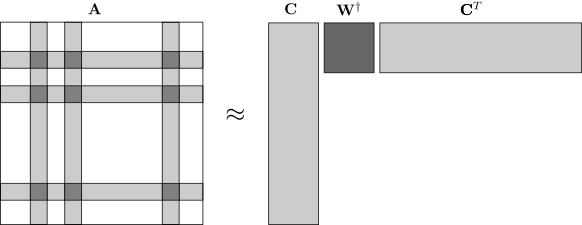
\includegraphics[scale=.75]{nystrom-procedure.pdf}
 % nystrom procedure.pdf: 466x180 pixel, 72dpi, 16.44x6.35 cm, bb=0 0 466 180
 \caption{The Nystr\"om extension procedure}
 \label{fig:nystromprocedure}
\end{figure}

The manner in which the columns are sampled and $\mat{W}^\pinv$ is calculated or approximated determines the type of the Nystr\"om extension. Various sampling schemes have been proposed, ranging from the simple scheme in which the columns are selected uniformly at random without replacement to more sophisticated and calculation-intensive schemes that involve sampling from a distribution determined by the determinants of principal submatrices of $\mat{A}$ \cite{BW09}. In practice the simple scheme represents a favorable trade-off between speed and accuracy \cite{KMT09}.
  
\subsection{Nystr\"om approximation of invariant subspaces}
In many applications, including the image-processing example taken from \cite{BCFM04}, the Nystr\"om extension is used to obtain approximations to the dominant eigenspaces of a real SPSD matrix $\mat{A},$ rather than a low-rank approximation \cite{homrighausen11}. In these applications the spectral norm approximation error is of interest, as it provides information on the quality of the approximate dominant eigenspaces obtained via Nystr\"om extensions. 

To be more precise, denote the $i$th-largest eigenvalue of an SPSD matrix $\mat{M}$ by $\lambda_i(\mat{M}),$ so that $\lambda_1(\mat{M}) \geq \lambda_2(\mat{M}) \geq \ldots.$ Let $\tilde{\mat{A}}$ be a Nystr\"om approximation to $\mat{A}$ and assume both $\mat{A}$ and $\tilde{\mat{A}}$ have well-defined dominant $k$-dimensional eigenspaces; that is, assume that $\lambda_{k}(\mat{A}) > \lambda_{k+1}(\mat{A})$ and likewise for $\tilde{\mat{A}}$. Let $\mat{U}_k$ and $\tilde{\mat{U}}_k$ have orthonormal columns and span, respectively, the dominant $k$-dimensional eigenspace of $\mat{A}$ and that of $\tilde{\mat{A}}.$ Recall one natural definition for the distance between these subspaces~\cite[Section 2.6.3]{GL96},  
\[
 \text{dist}(\mat{U}_k, \tilde{\mat{U}}_k) = \snorm{\mat{P}_{\mat{U}_k} - \mat{P}_{\tilde{\mat{U}}_k}} = \snorm{\mat{U}_k (\tilde{\mat{U}_k}^\perp)^\transp}.
\]
Here $\tilde{\mat{U}_k}^\perp$ is a matrix with orthonormal columns spanning the bottom $(n-k)$-dimensional eigenspace of $\tilde{\mat{A}}$ and $\mat{P}_{\mat{U}_k}$ ($\mat{P}_{\tilde{\mat{U}}_k}$) denotes the projection onto the span of $\mat{U}_k$ ($\tilde{\mat{U}}_k$).

Since $\mat{A}$ and $\tilde{\mat{A}}$ are both normal, it follows from \cite[Theorem VII.3.1]{Bhatia97} that 
\begin{equation}
 \text{dist}(\mat{U}_k, \tilde{\mat{U}}_k) \leq \frac{\snorm{\mat{A} - \tilde{\mat{A}}}}{\lambda_k(\mat{A}) - \lambda_{k+1}(\tilde{\mat{A}})} \leq \frac{\snorm{\mat{A} - \tilde{\mat{A}}}}{\lambda_k(\mat{A}) - \lambda_{k+1}(\mat{A}) - \snorm{\mat{A} - \tilde{\mat{A}}}}
\label{eqn:rawdksintheta}
\end{equation}
when $\lambda_k(\mat{A}) - \lambda_{k+1}(\mat{A}) - \snorm{\mat{A} - \tilde{\mat{A}}}$ is positive. Hence, if $\snorm{\mat{A} - \tilde{\mat{A}}}$ is smaller than the eigengap $\lambda_k(\mat{A}) - \lambda_{k+1}(\mat{A}),$ we can estimate the error in approximating the dominant $k$-dimensional eigenspace of $\mat{A}$ with that of $\tilde{\mat{A}}.$ This observation provides an additional motivation for seeking tighter bounds on the spectral error $\snorm{\mat{A} - \tilde{\mat{A}}}$ of the simple Nystr\"om extension.

\subsection{Our error bounds}The efficacy of the simple Nystr\"om extension is of course dependent on the data set to which it is applied. Intuitively, the extension should perform better if the information is spread evenly throughout the columns of the matrix. We use the concept of \emph{coherence}, taken from the matrix completion literature \cite{CR09}, to	provide a quantitative measure of the informativity of the columns of $\mat{A}.$ Let $\mathcal{S}$ be a $k$-dimensional subspace of $\R^n$ and $\mat{P}_{\mathcal{S}}$ denote the projection onto $\mathcal{S}.$ Then the coherence of $\mathcal{S}$ is
\[
 \mu(\mathcal{S}) = \frac{n}{k} \max\nolimits_i (\mat{P}_{\mathcal{S}})_{ii}.
\]
The coherence of the dominant $k$-dimensional eigenspace of $\mat{A}$ is a measure of how much comparative influence the individual columns of $\mat{A}$ have on this subspace: if $\mu$ is small, then all columns have essentially the same influence; if $\mu$ is large, then it is possible that there is a single column in $\mat{A}$ which alone determines one of the top $k$ eigenvectors of $\mat{A}.$ We mention that if $\mat{A}$ is rank-$k$, then the quantities $(\mat{P}_{\mathcal{S}})_{ii}$ are known to statisticians as the leverage scores of the columns of $\mat{A}$~\cite{DM10}.

For illustrative purposes, we point out that the coherence of a random $n \times k$ orthonormal matrix, i.e. a matrix distributed uniformly on the Stiefel manifold, is $\mathrm{O}(\max(k, \ln n)/k)$ with high probability~\cite[Lemma 2.2]{CR09}. The coherence of an arbitrary $k$-dimensional subspace is no smaller than $1,$ and may be as large as $n/k.$ 

Corollary~\ref{cor:simpleuniformnystromerror} is a condensed version of our main result, Theorem \ref{thm:uniformnystromerror}, and uses the notion of coherence to provide a bound on the error of the simple Nystr\"om extension. 

\begin{cor}
 Let $\mat{A}$ be a real SPSD matrix of size $n.$ Given an integer $k \leq n,$ let
$\mu$ denote the coherence of a dominant  $k$-dimensional invariant subspace of $\mat{A}.$
Fix a nonzero failure probability $\delta > 0.$ If $\ell \geq 8 \mu k \ln(k/\delta)$ columns of $\mat{A}$ are chosen uniformly at random without replacement, then 
\[
\snorm{\mat{A} - \mat{C} \mat{W}^\pinv \mat{C}^\transp} \leq \lambda_{k+1}(\mat{A}) \left(1 + \frac{2n}{\ell} \right) 
\]
with probability exceeding $1-\delta$ and
\[
 \snorm{\mat{A} - \mat{C} \mat{W}^\pinv \mat{C}^\transp} \leq \lambda_{k+1}(\mat{A}) + \frac{2}{\delta} \cdot \sum\nolimits_{i>k}\lambda_i(\mat{A})
\]
with probability exceeding $1 - 2\delta.$ If, additionally, $k \geq \rank(\mat{A}),$ then
\[
 \mat{A} = \mat{C} \mat{W}^\pinv \mat{C}^\transp
\]
with probability exceeding $1-\delta.$


\label{cor:simpleuniformnystromerror}
\end{cor}
The dependence of the relative error bound provided in Corollary~\ref{cor:simpleuniformnystromerror} is optimal on $n$ and $\ell;$ this is established in Section~\ref{sec:naiveproof}.

For Corollary \ref{cor:simpleuniformnystromerror} to provide a meaningful estimate of $\ell,$ the required number of column samples, the coherence must be small enough that $\ell \ll n.$ This requirement reflects our intuition that approximations formed using a small number of columns will not be accurate if a small number of columns are significantly more influential than the others. In the best-case scenario of $\mu=1,$ the columns are equally informative and we find that the error of a simple Nystr\"om extension formed using just $8 k \ln (k/\delta)$ columns is a bounded multiple of the error of the optimal rank-$k$ approximation. Furthermore, we see that the efficacy of the simple Nystr\"om extension increases in the presence of spectral decay. If the eigenvalues of $\mat{A}$ decay sufficiently then the error of the simple Nystr\"om extension may even be bounded by a small multiple of the error of the optimal rank-$k$ approximation.

\subsection{Stable algorithms}
\label{sec:stablealgs}
In general, the computation of the simple Nystr\"om extension is unstable because it requires one to take the pseudoinverse of a matrix $\mat{W}$ which may be nearly singular. The product $\mat{W}^\pinv \mat{C}^\transp$ can be computed stably if the condition number $\kappa(\mat{W}) = \lambda_1(\mat{W})/\lambda_\ell(\mat{W})$ is small (here $\mat{W}$ is an $\ell\times\ell$ matrix)~\cite{GL96}. The maximum eigenvalue of $\mat{W}$ is smaller\footnote{Matrix concentration inequalities can be used to estimate $\lambda_1(\mat{W})$ more precisely; see e.g.~\cite{T10,MJCFT12}.} than that of $\mat{A},$ so when the minimum eigenvalue of $\mat{W}$ is sufficiently bounded away from zero the condition number of $\mat{W}$ is small and the simple Nystr\"om extension can be stably computed. If we do not have \emph{a priori} knowledge that the condition number of $\mat{W}$ is small, one should instead compute an approximation to the simple Nystr\"om extension using an algorithm that ensures that $\lambda_\ell(\mat{W})$ is not small. We propose two such algorithms.

Algorithm~\ref{alg:simple-stable-nystrom} returns a simple Nystr\"om extension of $\mat{A}_\rho := \mat{A} + \rho \mat{I}$ for some small positive constant $\rho.$ Since $\mat{A}_\rho$ has a minimum eigenvalue bounded away from zero by at least $\rho,$ the computation of the simple Nystr\"om extension is stable: one can use, for instance, a Cholesky decomposition to compute the required inversion stably.
\begin{algorithm}
 \caption{Nystr\"om extension of a regularized $\mat{A}$}
 \label{alg:simple-stable-nystrom}
 \algrenewcommand\algorithmicrequire{\textbf{Input:}}
 \algrenewcommand\algorithmicensure{\textbf{Output:}}
 \begin{algorithmic}[1]
  \Require{ $\mat{A}$, an $n \times n$ SPSD matrix; an integer $k \in [1,n];$ a regularization parameter $\rho > 0;$ and an integer $\ell \geq k.$ }
  \Ensure{$\mat{C}_\rho$, an $n \times \ell$ matrix; and $\mat{W}_\rho$, an $\ell \times \ell$ SPSD matrix.}	
  \Statex
  
 \State Let $\mat{A}_\rho = \mat{A} + \rho \mat{I}.$
 \State Uniformly select, without replacement, $\ell$ indices in $\{1,\ldots,n\}$ and let $\mat{S} \in \R^{n \times \ell}$ be the corresponding column selector matrix. That is, let $(\mat{S})_{i,j} = 1$ if $i$ was the $j$th index selected, and $(\mat{S})_{i,j} = 0$ otherwise.
 \State Form the matrix $\mat{C}_\rho = \mat{A}_\rho \mat{S}.$
 \State Form the matrix $\mat{W}_\rho = \mat{S}^\transp \mat{A}_\rho \mat{S}.$
  \end{algorithmic}

\end{algorithm}

Algorithm~\ref{alg:stable-nystrom} returns a Nystr\"om extension where the matrix $\mat{C}$ is taken from $\mat{A},$ but the coupling matrix $\mat{W}_\rho$ is taken from $\mat{A}_\rho.$ Intuitively, for small $\rho,$ the approximation returned by Algorithm~\ref{alg:stable-nystrom}, $\mat{C}\mat{W}_\rho^{-1} \mat{C}^\transp,$ should be a better approximation to $\mat{A}$ than that returned by Algorithm~\ref{alg:simple-stable-nystrom}, $\mat{C}_\rho \mat{W}_\rho^{-1} \mat{C}_\rho^\transp,$ because it uses more information from $\mat{A}.$ However, it is not clear that this intuition should hold for larger $\rho$: the added accuracy from using $\mat{C}$ may be negated by the fact that $\mat{C}$ and $\mat{W}_\rho$ are from two different matrices, so $\mat{C}\mat{W}_\rho^{-1} \mat{C}^\transp$ can no longer be thought of as a Nystr\"om extension of a matrix close to $\mat{A},$ whereas $\mat{C}_\rho \mat{W}_\rho^{-1} \mat{C}_\rho^\transp$ is always a Nystr\"om extension of a matrix that is close to $\mat{A}.$

\begin{algorithm}
 \caption{Nystr\"om extension using a regularized coupling matrix}
 \label{alg:stable-nystrom}
 \algrenewcommand\algorithmicrequire{\textbf{Input:}}
 \algrenewcommand\algorithmicensure{\textbf{Output:}}
 \begin{algorithmic}[1]
  \Require{  $\mat{A},$ an $n \times n$ SPSD matrix; an integer $k \in [1,n];$ a tolerance $\rho > 0;$ and an integer $\ell \geq k.$ }
  \Ensure{$\mat{C}$, an $n \times \ell$ matrix; and $\mat{W}_\rho,$ an $\ell \times \ell$ SPSD matrix.}
  \Statex
  
 \State Uniformly select, without replacement, $\ell$ indices in $\{1,\ldots,n\}$ and let $\mat{S} \in \R^{n \times \ell}$ be the corresponding column selector matrix. That is, let $(\mat{S})_{i,j} = 1$ if $i$ was the $j$th index selected, and $(\mat{S})_{i,j} = 0$ otherwise.
 \State Form the matrix $\mat{C} = \mat{A} \mat{S}.$
 \State Form the matrix $\mat{W} = \mat{S}^\transp \mat{A} \mat{S}.$
 \State If $\lambdamin{\mat{W}} \geq \rho,$ then take $\mat{W}_\rho = \mat{W},$
 \Statex otherwise take $\mat{W}_\rho = \mat{W} + \rho \mat{I}.$
 \end{algorithmic}

\end{algorithm}

The cost of forming the Nystr\"om extension returned by each of these algorithms is $\const{O}(\ell^3 + \ell^2 n).$ We have the following accuracy guarantees.

\begin{thm}
 Let $\mat{A}$ be a real SPSD matrix of size $n.$ Given an integer $k \leq n$ and a tolerance $\rho >0,$ let
$\mu$ denote the coherence of a dominant  $k$-dimensional invariant subspace of $\mat{A}.$
Fix a nonzero failure probability $\delta.$ 

If $\ell \geq 8 \mu k \ln(k/\delta)$ then the Nystr\"om extension returned by Algorithm~\ref{alg:simple-stable-nystrom} satisfies 
\[
  \snorm{\mat{A} - \mat{C}_\rho\mat{W}_\rho^{-1} \mat{C}_\rho^\transp } \leq \lambda_{k+1}(\mat{A})\left(1 + \frac{2n}{\ell}\right) + \frac{2 \rho n}{\ell} + \rho.
\]
with probability at least $1- \delta$ and
\[
 \snorm{\mat{A} - \mat{C}_\rho\mat{W}_\rho^{-1} \mat{C}_\rho^\transp } \leq \lambda_{k+1}(\mat{A}) + \frac{2}{\delta} \sum\nolimits_{i=k+1}^n \lambda_i(\mat{A}) + \frac{2\rho (n-k)}{\delta} + 2\rho
\]
with probability at least $1 - 2\delta.$

Likewise, if $\ell \geq 8 \mu k \ln(k/\delta)$ then the Nystr\"om extension returned by Algorithm~\ref{alg:stable-nystrom} satisfies
\[
  \snorm{\mat{A} - \mat{C}\mat{W}_\rho^{-1} \mat{C}^\transp } \leq \lambda_{k+1}(\mat{A}) \left(3 + \frac{2n}{\ell}\right) + \frac{2 \rho n}{\ell} + 4\rho\sqrt{\frac{ n}{\ell}} + 5\rho
\]
with probability at least $1- \delta$ and
\[
 \snorm{\mat{A} - \mat{C}\mat{W}_\rho^{-1} \mat{C}^\transp } \leq 3 \lambda_{k+1}(\mat{A}) + \frac{2}{\delta} \sum\nolimits_{i=k+1}^n \lambda_i(\mat{A}) + \frac{2 \rho (n-k)}{\delta} + 4\rho\sqrt{\frac{n}{\ell}} + 5\rho
\]
with probability at least $1 - 2\delta.$
\label{thm:stabilized-nystrom-error-bounds}
\end{thm}



\subsection{Relevant literature}
% \begin{table}[t]
% \caption{Simple Nystr\"om extension error guarantees}
% \tiny
% \begin{flushleft}
% Summary of prior guarantees on the performance of the simple Nystr\"om extension. Given an $n \times n$ positive semidefinite matrix $\mat{A},$ we compare the error of the simple Nystr\"om extension to the error of the optimal rank-$k$ approximation in the spectral and Frobenius norms. Let the diagonal matrix $\mat{\Sigma}_2$ contain the bottom $n-k$ eigenvalues of $\mat{A}$. Then these optimal errors are given by $\|\mat{\Sigma}_2\|_2$ and $\|\mat{\Sigma}_2\|_F$ respectively. Notation: $(\cdot)$ denotes the difference between $\mat{A}$ and the Nystr\"om extension, $\ell$ is the number of column samples used, the columns of $\mat{U}_1$ comprise the top $k$ eigenvectors of $\mat{A},$ and $\sum_{i=1}^\ell a_{ii}^\downarrow$ is the sum of the $\ell$ largest entries on the diagonal of $\mat{A}.$
% \end{flushleft}
% \begin{tabular}{l c c p{1.5in}}
% \hline
% Source & Guarantees & $\ell$ & Remarks \\
% \hline  
% \cite{KMT09}			& $\E\|\cdot\|_F \leq \|\mat{\Sigma}_2\|_F + \varepsilon\left(\left(\frac{n}{\ell} \sum_{i=1}^\ell a_{ii}^\downarrow \right) \sqrt{n \sum_{i=1}^n a_{ii}^2} \right)^{1/2}$ & $64 \varepsilon^{-4} k$ & sampling without replacement  \\
% \cite{TR10}			& $\|\cdot\|_2 = \|\cdot\|_F = 0$	& $\mathrm{O}(n \max_{ij} |(\mat{U}_1)_{ij}|^2 k \ln(k) )$ & sampling with replacement, constant probability of success, requires $\rank(\mat{A})=k$\\
% \multirow{2}{*}{\cite{KLL10}}			& $\E\|\cdot\|_2 \leq \Omega(1) \|\mat{\Sigma}_2\|_2 + \Omega\left(\frac{n}{\sqrt{\ell}}\right) \max_i a_{ii}$ & $\mathrm{O}(k)$ & \multirow{2}{*}{large scale variant, with replacement} \\
% 	& $\E\|\cdot\|_F \leq \Omega(\sqrt{k}) \|\mat{\Sigma}_2\|_F + \Omega(n)\max_i a_{ii}$ & $\mathrm{O}(k)$ & \\
% \cite{MTJ11}                   & $\|\cdot\|_F \leq (1+\varepsilon)\|\mat{\Sigma}_2\|_F$                                                       & $\mathrm{O}( \varepsilon^{-2} n \max_i |(\mat{U}_1)_{i}|^2 \ln(k))$ & sampling without replacement, constant probability of success
% \end{tabular}
% \label{tab:previousresults}
% \end{table}

We survey the literature on CUR decompositions and Nystr\"om extensions, focusing on the simple Nystr\"om scheme. Discussion of the column subset selection literature is deferred to Section~\ref{sec:colselection}, after the connection between the Nystr\"om extension procedure and the column subset selection problem is made explicit. In this section $\mat{A}$ is an $n \times n$ SPSD matrix, $\mat{A}_k$ is a rank-$k$ approximation to $\mat{A}$ that is optimal in the spectral norm, $\ell$ is the number of columns used to construct a Nystr\"om extension of $\mat{A}, $ $\delta \in (0,1)$ is a failure probability, and $\varepsilon > 0$ is an accuracy parameter.

In \cite{GTZ97}, Goreinov, Tyrtyshnikov, and Zamarashkin introduce deterministic CUR decompositions under the name pseudo-skeleton approximations. They establish that there exists at least one set of exactly $k$ columns and $k$ rows for which the corresponding pseudo-skeleton approximation has a spectral norm error smaller than $\snorm{\mat{A} - \mat{A}_k} (1 +4 \sqrt{k n}).$ Finding these columns and rows is connected to the problem of finding a $k \times k$ submatrix of $\mat{A}$ whose determinant has the maximal modulus~\cite{GTZ97ii}.

Drineas, Kannan, and Mahoney \cite{DKM06} show that if appropriate probability distributions are used to select the columns and rows, the accuracy of the resulting CUR approximations does not depend on the dimensions $k$ and $n.$ Specifically, if the columns and rows are sampled with probability proportional to their Euclidean norms, then the spectral and Frobenius norm errors of the approximations are within an additive factor of $\varepsilon \|\mat{A}\|_F$ of the optimal errors. Let $c$ and $r$ denote the number of columns and rows sampled to form $\mat{C}$ and $\mat{R}$ respectively, then 
\begin{align*}
 \snorm{\mat{A} - \mat{C} \mat{U} \mat{R}} & \leq \snorm{\mat{A} - \mat{A}_k} + \varepsilon \fnorm{\mat{A}} \\
 \fnorm{\mat{A} - \mat{C} \mat{U} \mat{R}} & \leq \fnorm{\mat{A} - \mat{A}_k} + \varepsilon \fnorm{\mat{A}}
\end{align*}
with probability at least $1-\delta$ when $c = \Omega(k\varepsilon^{-4} \ln \delta^{-1})$ and $r = \Omega(k\varepsilon^{-2}\delta^{-2}).$ The coupling matrix $\mat{U}$ is computed from $\mat{C}$ and $\mat{R}.$

 In \cite{DMM08CUR}, Drineas, Mahoney, and Muthukrishnan propose forming CUR decompositions by using ``subspace sampling'' probabilities that capture the influence of the columns of $\mat{A}$ on the top $k$-dimensional eigenspace of $\mat{A}$: if $\mat{P}$ is the projection onto this eigenspace, then the probability of selecting the $i$th column is taken to be proportional to $(\mat{P})_{ii}.$ Later works refer to these probabilities as leverage score probabilities to emphasize their connection to the leverage scores encountered in linear regression problems~\cite{DM09,DM10}. \cite{DMM08CUR} gives a $(1+\epsilon)$ Frobenius norm relative-error guarantee on the quality of the CUR approximations: if $c = \Omega(k^2 \varepsilon^{-2} \ln \delta^{-1} )$ columns are sampled from $\mat{A}$ with replacement according to the leverage score distribution of $\mat{A}$ and $r = \Omega(c^2 \varepsilon^{-2} \ln \delta^{-1})$ rows are then sampled from $\mat{A}$ according to the leverage score distribution of $\mat{C}^\transp$, then
\[
 \fnorm{\mat{A} - \mat{C} \mat{U}\mat{R}} \leq (1 + \varepsilon) \fnorm{\mat{A} - \mat{A}_k}
\]
with probability at least $1-\delta.$ Here the coupling matrix $\mat{U}$ is the pseudoinverse of the intersection between $\mat{R}$ and $\mat{C}.$ 

%, but computing these probabilities seems to be as expensive as computing the rank-$k$ truncated SVD.

Williams and Seeger introduce the Nystr\"om extension in \cite{SW01}, based upon a similar method used in numerical integral equation solvers, as a heuristic method for efficiently approximating the eigendecomposition of kernel matrices. % In this seminal work, only an empirical analysis of the approximation error is offered.
Drineas and Mahoney provide the first rigorous analysis of a Nystr\"om extension in \cite{DM05}; in the scheme they consider, columns are sampled with probability proportional to the square of the diagonal entries of $\mat{A}$. They show that if $\mat{C}$ is constructed by sampling $\Omega(k \varepsilon^{-4} \ln\delta^{-1})$ columns with replacement from this distribution, then
\begin{align*}
\snorm{\mat{A} - \mat{C} \mat{W}^\pinv \mat{C}^\transp} & \leq \snorm{\mat{A} - \mat{A}_k} + \varepsilon \sum_{k=1}^n (\mat{A})_{ii}^2 \\
\fnorm{\mat{A} - \mat{C} \mat{W}^\pinv \mat{C}^\transp} & \leq \fnorm{\mat{A} - \mat{A}_k} + \varepsilon \sum_{k=1}^n (\mat{A})_{ii}^2
\end{align*}
with probability at least $1-\delta$~\cite{DM05}. In addition to probabilistic schemes, many adaptive sampling schemes have been proposed. These attempt to progressively choose the columns to decrease the approximation error. For an introduction to this body of literature, we refer the interested reader to the discussion in \cite{FGK11}.

Kumar, Mohri, and Talwalkar attempt the first analysis of the simple Nystr\"om extension in \cite{KMT09}, resulting in bounds for the Frobenius norm error. Their analysis proceeds by bounding the expectation and variance of the error then applying a concentration of measure argument. A simplified yet representative statement of their bound is that 
\[
 \fnorm{\mat{A} - \mat{C}\mat{W}^\pinv\mat{C}^\transp} \leq \fnorm{\mat{A} - \mat{A}_k} + \varepsilon n \cdot \max_i {(\mat{A})_{ii}}
\]
with probability at least $1-\delta$ when $\ell = \Omega(k \varepsilon^{-4}\ln \delta^{-1}).$ 

In \cite{KMT09a}, Kumar, Mohri, and Talwalkar establish that if $\text{rank}(\mat{W})= \text{rank}(\mat{A}) = k,$ then $\mat{A} = \mat{C}\mat{W}^\pinv \mat{C}^\transp.$ Talwalkar and Rostamizadeh prove this implies that, if $\ell = \Omega(k \tau \ln(k/\delta))$, simple Nystr\"om extension results in exact recovery with probability at least $1-\delta$ \cite{TR10}. That is, if $\ell$ is sufficiently large, then the Nystr\"om extension is exactly $\mat{A}.$ Here $\tau$ is a different measure of the coherence of the top $k$-dimensional eigenspace of $\mat{A}$ than is used in this paper: let the columns of $\mat{U}_1$ be the normalized top $k$ eigenvectors of $\mat{A},$ then $ \tau = n \max_{i,j} \big(\mat{U}_1\big)_{ij}^2.$ Their key observation is that if no columns of $\mat{A}$ are singularly influential, then $\mat{W}$ will have maximal rank when $\ell$ is slightly larger than the rank of $\mat{A}$. Thus, the number of samples required for exact recovery is determined by the rank of $\mat{A}$ and the 
coherence, $\tau,$ of its range space. They use a standard result from the compressed sensing literature to quantify this phenomenon and obtain an estimate for $\ell$ \cite{CR07}.

  In \cite{KLL10}, Kwok, Li, and Lu propose replacing $\mat{W}$ with a low-rank approximation $\tilde{\mat{W}}$ to facilitate the pseudoinversion operation. This large-scale variant of the simple Nystr\"om extension allows a larger number of column samples to be drawn and leads to smaller empirical approximation errors. The approximation $\tilde{\mat{W}}$ is constructed using the randomized methodology espoused in \cite{HMT11}. Namely, to construct $\tilde{\mat{W}},$ one first forms the product $\mat{Y} = \mat{W}^{q} \mat{\Omega}$ by applying $\mat{W}$ multiple times to a random $\ell \times (k+p)$ matrix $\mat{\Omega}$ whose entries are standard Gaussian random variables. Intuitively, the range space of $\mat{Y}$ captures the top $k$-dimensional eigenspace of $\mat{W},$ so to form $\tilde{\mat{W}}$ one lets $\mat{Q}$ be an orthonormal basis for the range space of $\mat{Y}$ and takes $\tilde{\mat{W}} = \mat{Q}\mat{Q}^\transp \mat{W} \mat{Q}\mat{Q}^\transp$ to be the restriction of $\mat{W}$ to the range 
space of $\mat{Y}.$ The pseudoinverse of $\tilde{\mat{W}}$ is potentially much cheaper to compute than that of $\mat{W},$ since one only has to invert a smaller $k+p$ matrix: $\tilde{\mat{W}}^\pinv = \mat{Q} (\mat{Q}^\transp \mat{W} \mat{Q})^\pinv \mat{Q}^\transp.$  

 The analysis of Kwok et al.'s scheme combines bounds provided in \cite{HMT11} with a matrix sparsification argument. In addition to $\ell$ and $k$, the Nystr\"om algorithm presented in \cite{KLL10} depends on two additional parameters that control the creation of $\tilde{\mat{W}}$: the oversampling factor $p$ and the number of iterations $q.$ 
%For simplicity we set $p = k;$ with this choice the error bounds in \cite{KLL10} reduce to
% \begin{align*}
%  \E\| \mat{A} - \mat{C}\mat{W}^\pinv \mat{C}^\transp\|_2 & \leq C  \left(\frac{\ell}{k}\right)^{1/q} \left(\|\mat{A} - \mat{A}_k\|_2 + \frac{n}{\sqrt{l}} \max_i \mat{A}_{ii} \right) \\
%  \E\| \mat{A} - \mat{C}\mat{W}^\pinv \mat{C}^\transp\|_F & \leq C \sqrt{k} \left( \|\mat{A} - \mat{A}_k\|_F + \frac{n}{\sqrt{\ell}} \max_i \mat{A}_{ii} \right).
% \end{align*}
The results of \cite{KLL10} provide error bounds for the simple Nystr\"om extension (take $p = \ell -k$ and $q=1$):
\begin{align}
 \E\| \mat{A} - \mat{C}\mat{W}^\pinv \mat{C}^\transp\|_2 & \leq \const{C} \left(\|\mat{A} - \mat{A}_k\|_2 + \frac{n}{\sqrt{\ell}} \max_i (\mat{A})_{ii} \right) \label{eqn:kll10spectralbound}\\
 \E\| \mat{A} - \mat{C}\mat{W}^\pinv \mat{C}^\transp\|_F & \leq \const{C} \big( \sqrt{\ell} \cdot \|\mat{A} - \mat{A}_k\|_F + n \cdot \max_i (\mat{A})_{ii} \big). \notag
\end{align}
Here the constant $\const{C}$ depends on the relationship between $k$ and $\ell;$ if, e.g., $\ell = k \ln k$ and $k > 6$ then $\const{C}$ can be taken to be 8. 

Of the works mentioned, only \cite{KLL10} provides a bound on the spectral error of the simple Nystr\"om extension for $\mat{A}$ of arbitrary rank. Unfortunately, the quantity $\max_i (\mat{A})_{ii}$ is, for a general SPSD $\mat{A},$ bounded only by $\lambda_1(\mat{A}).$ Thus equation \eqref{eqn:kll10spectralbound} does not provide a relative-error bound. In fact, the spectral norm error bound provided in this paper is always tighter than the bound provided in \cite{KLL10}, for any choice of $p$ and $q.$ 
 
Most recently, in a simultaneously completed work, Chiu and Demanet consider CUR decompositions of rectangular matrices that are formed by sampling uniformly at random with replacement from the columns and rows of the matrix~\cite{CD11}. Using a different technique, they establish bounds similar to those given in Theorem~\ref{thm:stabilized-nystrom-error-bounds}. Their proposed CUR algorithm, applied to SPSD matrices, sets the eigenvalues of $\mat{W}$ that are smaller than $\rho$ to zero, thereby ensuring that $\snorm{\mat{W}^\pinv} \leq \rho^{-1}$ and allowing the Nystr\"om extension to be computed stably (see Section~\ref{sec:stablealgs}). 

The results in~\cite{CD11} imply that if $\rho = \lambda_{k+1}(\mat{A})$ then, with high probability, the error of a Nystr\"om extension constructed using this algorithm stays within a multiplicative $\mathrm{O}(n/\ell)$ factor of the optimal rank-$k$ approximation error. We note that Theorem~\ref{thm:stabilized-nystrom-error-bounds} gives the same guarantee for Algorithms~\ref{alg:simple-stable-nystrom} and~\ref{alg:stable-nystrom} for the same choice of $\rho.$ However, in general one does not know $\lambda_{k+1}(\mat{A}),$ so it is instructive to compare the bounds from~\cite{CD11} with our bounds, for arbitrary regularization parameters $\rho.$ According to the first bound in Theorem~\ref{thm:stabilized-nystrom-error-bounds}, the error of the extensions 
calculated by Algorithms~\ref{alg:simple-stable-nystrom} and~\ref{alg:stable-nystrom} is on the order of
\[
 (\lambda_{k+1}(\mat{A}) + \rho)\frac{n}{\ell},
\]
while the corresponding bound for the algorithm proposed in~\cite{CD11} has an error on the order of
\[
 \bigg(\lambda_{k+1}(\mat{A}) + \rho + \frac{\lambda_{k+1}(\mat{A})^2}{\rho}\bigg)\frac{n}{\ell},
\]
which may be much larger when $\rho < \lambda_{k+1}(\mat{A}).$

In contrast to prior work, this work (concurrently with~\cite{CD11}) supplies the first truly relative error spectral norm approximation guarantee for the simple Nystr\"om approximation, and establishes an explicit connection between the coherence of the dominant $k$-dimensional eigenspace of the matrix and the number of column samples needed to obtain this guarantee. A spectral norm error bound is also provided that, in the presence of spectral decay, gives smaller additive error than available in the current literature. We show the optimality of the dependence of the relative error bound on the dimension of the matrix and the number of column samples used in forming the Nystr\"om extension.

Our results are obtained by establishing an explicit connection between the randomized column subset selection problem and the quality of Nystr\"om extensions.  This connection is of independent interest, as it implies that any guarantee on the error of randomized column subset selection directly implies a matching guarantee on the error of Nystr\"om extension, and vice versa. While this paper considers only the spectral norm error of the simple Nystr\"om extension scheme, we believe the framework given is flexible enough to be fruitfully applied to the analysis of errors measured in other norms and of other Nystr\"om schemes including, in particular, the large-scale variant introduced in~\cite{KLL10}.

\subsection{Outline} In Section~\ref{sec:notation} we introduce our notation and review some algebraic preliminaries. In Section~\ref{sec:colselection} we establish a connection between the Nystr\"om extension procedure and the column subset selection problem. We exploit this connection and a result from~\cite{HMT11} to provide a general error bound for any Nystr\"om extension scheme. In Section~\ref{sec:naiveproof} we specialize this result to the case of the simple Nystr\"om extension. We conclude with an empirical investigation of Algorithms~\ref{alg:simple-stable-nystrom} and~\ref{alg:stable-nystrom} in Section~\ref{sec:experiments}.

\section{Notation}
\label{sec:notation}

We work exclusively with real matrices and order the eigenvalues of a SPSD matrix $\mat{A}$ so that $\lambda_1(\mat{A}) \geq \lambda_2(\mat{A}) \geq \cdots \geq \lambda_n(\mat{A}).$ Each SPSD matrix $\mat{A}$ has a unique square root $\mat{A}^{1/2}$ that is also symmetric positive-semidefinite, has the same eigenspaces as $\mat{A},$ and satisfies $\mat{A} = \big(\mat{A}^{1/2}\big)^2.$ We write $\mat{A} \succeq \mat{B}$ if $\mat{A} - \mat{B}$ is SPSD.

The projection onto the column space of a matrix $\mat{M}$ is written $\mat{P}_{\mat{M}}$ and satisfies
\[
\mat{P}_{\mat{M}} = \mat{M}\mat{M}^\pinv = \mat{M} (\mat{M}^\transp \mat{M})^\pinv \mat{M}^\transp.
\]
The notation $(\vec{x})_j$ refers to the $j$th entry of the vector $\vec{x},$ and $(\mat{M})_i$ refers to the $i$th column of the matrix $\mat{M}.$ Likewise, $(\mat{M})_{ij}$ refers to the $(i,j)$ entry of $\mat{M}.$

The coherence of a matrix $\mat{U} \in \R^{n\times k}$ with orthonormal columns is the coherence of the subspace $\mathcal{S}$ which it spans:
\[
\mu(\mat{U}) := \mu(\mathcal{S}) = \frac{n}{k} \max\nolimits_i (\mat{P}_{\mathcal{S}})_{ii} = \frac{n}{k} \max\nolimits_i (\mat{U}\mat{U}^\transp)_{ii}.
\]
\section{The connection to the column subset selection problem}
\label{sec:colselection}

In this section we establish a fruitful connection between the performance of the Nystr\"om extension and the performance of randomized \emph{column subset selection}.
% Prior analyses of Nystr\"om extensions have used the Cholesky decomposition. 

Given a matrix $\mat{M}$, the goal of column selection is to choose a small but informative subset $\mat{C}$ of the columns of $\mat{M}.$ Informativity can be defined in many ways; in our context, $\mat{C}$ is informative if, after approximating $\mat{M}$ with the matrix obtained by projecting $\mat{M}$ onto the span of $\mat{C},$ the residual $(\mat{I} - \mat{P}_{\mat{C}})\mat{M}$ is small in some norm. In randomized column subset selection, the columns $\mat{C}$ are chosen randomly, either uniformly or according to some data-dependent distribution. Column subset selection has important applications in statistical data analysis and has been investigated by both the numerical linear algebra and the theoretical computer science communities. For an introduction to the column subset selection literature biased towards approaches involving randomization, we refer the interested reader to the surveys \cite{MM10,MM11}.

Our first theorem establishes that the Nystr\"om extension of $\mat{A}$ is intimately related to the randomized column subset selection problem for $\mat{A}^{1/2}.$
We model the column sampling operation as follows: let $\mat{S}$ be a random matrix with $\ell$ columns, each of which has exactly one nonzero element. Then right multiplication by $\mat{S}$ selects  $\ell$ columns from $\mat{A}$:
\begin{equation*}
  \mat{C} = \mat{A} \mat{S} \quad \text{ and } \quad \mat{W} = \mat{S}^\transp \mat{A} \mat{S}.
\end{equation*}
The distribution of $\mat{S}$ reflects the type of sampling being performed. In the case of the simple Nystr\"om extension,  $\mat{S}$ is distributed as the first $\ell$ columns of a matrix sampled uniformly at random from the set of all permutation matrices.

We use the following partitioning of the eigenvalue decomposition of $\mat{A}$ to state our results:
\begin{equation}
\mat{A} = \bordermatrix[{[}{]}]{%
&^k \vspace{-0.75ex} & \!\!^{n-k}  \hspace{1ex}\\
& \vspace{0.25ex} \mat{U}_1 \hspace{-2ex} & \mat{U}_2 
}
\bordermatrix[{[}{]}]{%
& \vspace{-0.75ex} ^k &\!\!^{n-k} \hspace{1ex}\\
& \mat{\Sigma}_1 & \\
& \vspace{0.5ex} & \mat{\Sigma}_2 
}
\bordermatrix*[{[}{]}]{%
\mat{U}_1^\transp \!\! & \\
\vspace{-1ex} \mat{U}_2^\transp \!\! & \\
 \vspace{-1ex} &
}
\label{eqn:svdpartition}
\end{equation}


The matrix $[\mat{U}_1\  \mat{U}_2]$ is orthogonal, $\mat{\Sigma}_1$ contains the $k$ largest eigenvalues of $\mat{A},$ and the columns of $\mat{U}_1$ and $\mat{U}_2$ respectively span a dominant $k$-dimensional invariant subspace of $\mat{A}$ and the corresponding bottom $(n-k)$-dimensional invariant subspace of $\mat{A}.$ The interaction of the column sampling matrix $\mat{S}$ with the invariant subspaces spanned by $\mat{U}_1$ and $\mat{U}_2$ is captured by the matrices
\begin{equation}
 \mat{\Omega}_1 = \mat{U}_1^\transp \mat{S}, \quad \mat{\Omega}_2 = \mat{U}_2^\transp \mat{S}.
\label{eqn:sampleprojections}
\end{equation}

\begin{thm}
Let $\mat{A}$ be an SPSD matrix of size $n$ and let $\mat{S}$ be an $n \times \ell$ matrix. Partition $\mat{A}$ as in equation \eqref{eqn:svdpartition} and define $\mat{\Omega}_1$ and $\mat{\Omega}_2$ as in equation \eqref{eqn:sampleprojections}.

Assume $\mat{\Omega}_1$ has full row rank. Then the spectral approximation error of the Nystr\"om extension of $\mat{A}$ using $\mat{S}$ as the column sampling matrix satisfies
\begin{equation}
\|\mat{A} - \mat{C}\mat{W}^\pinv \mat{C}^\transp\|_2 = \|\big(\mat{I} - \mat{P}_{\mat{A}^{1/2} \mat{S}}\big)\mat{A}^{1/2}\|_2^2 \leq \norm{\mat{\Sigma}_2}_2 + \|\mat{\Sigma}_2^{1/2} \mat{\Omega}_2 \mat{\Omega}_1^\pinv\|_2^2.
  \label{eqn:spectralnystromerrbound}
\end{equation}
If $\rank(\mat{A}) < k,$ then in fact
\[
 \mat{A} = \mat{C}\mat{W}^\pinv \mat{C}^\transp.
\]
\label{thm:colselection}
\end{thm}


%Theorem \ref{thm:colselection} establishes an equivalence between the column subset selection problem and the Nystr\"om extension procedure and gives a deterministic relative-error bound on the performance of Nystr\"om extensions. 

\begin{remark}
We emphasize that the first relation in \eqref{eqn:spectralnystromerrbound} is an equality. That is, the spectral norm error of approximating $\mat{A}$ with a Nystr\"om extension is exactly the square of the spectral norm error of approximating $\mat{A}^{1/2}$ with a specific corresponding low-rank approximant. 

In fact, this equality holds when $\mat{A}^{1/2}$ is replaced with any generalized Cholesky factorization of $\mat{A}$: by appropriately modifying the proof of Theorem~\ref{thm:colselection}, it can be seen that if $\mat{P} \mat{A} \mat{P}^\transp = \mat{B}^\transp \mat{B}$ where $\mat{P}$ is a permutation matrix, then 
\[
 \snorm{\mat{A} - \mat{C}\mat{W}^\pinv \mat{C}^\transp} = \snorms{(\mat{I} - \mat{P}_{\mat{B}\mat{P}\mat{S}})\mat{B}}
\]
as well. We take $\mat{P} = \mat{I}$ and $\mat{B} = \mat{A}^{1/2}$ in this paper.
\end{remark}

To establish Theorem \ref{thm:colselection}, we use the following bound on the error incurred by projecting a matrix onto a random subspace of its range (\cite[Theorem 9.1]{HMT11}).

\begin{prop}
 Let $\mat{M}$ be an SPSD matrix of size $n$. Fix integers $k$ and $\ell$ satisfying $1 \leq k \leq \ell \leq n.$ 

Let $\mat{U}_1$ and $\mat{U}_2$ be matrices with orthonormal columns spanning, respectively, a dominant $k$-dimensional eigenspace of $\mat{M}$ and the corresponding bottom $(n-k)$-dimensional eigenspace of $\mat{M}.$ Let $\mat{\Sigma}_1$ and $\mat{\Sigma}_2$ be the diagonal matrices of eigenvalues corresponding, respectively, to the dominant $k$-dimensional eigenspace of $\mat{M}$ and the bottom $(n-k)$-dimensional eigenspace of $\mat{M}.$ 

Given a matrix $\mat{S}$ of size $n \times \ell$, define $\mat{\Omega_1} = \mat{U}_1^\transp \mat{S}$ and $\mat{\Omega_2} = \mat{U}_2^\transp \mat{S}.$ Then, assuming that $\mat{\Omega}_1$ has full row rank,
\[
\| (\mat{I} - \mat{P}_{\mat{M}\mat{S}}) \mat{M} \|_2^2 \leq \| \mat{\Sigma}_2 \|_2^2 + \big\| \mat{\Sigma}_2 \mat{\Omega}_2 \mat{\Omega}_1^\pinv \big \|_2^2.
\]
If, additionally, $\mat{\Sigma}_1$ is singular, then
\[
 \mat{M} = \mat{P}_{\mat{M}\mat{S}}\mat{M}.
\]

 \label{prop:deterministicerrorbound}
\end{prop}

\begin{proof}[Proof of Theorem \ref{thm:colselection}]
We write the Nystr\"om extension in terms of the square root of $\mat{A}$ and a projection onto the space spanned by $\mat{A}^{1/2} \mat{S}:$
\begin{align*}
  \mat{C} \mat{W}^\pinv \mat{C}^\transp & = \mat{A} \mat{S} (\mat{S}^\transp \mat{A} \mat{S})^\pinv \mat{S}^\transp \mat{A} \\
  & = \mat{A}^{1/2} [\mat{A}^{1/2} \mat{S} (\mat{S}^\transp \mat{A}^{1/2} \mat{A}^{1/2} \mat{S})^\pinv \mat{S}^\transp \mat{A}^{1/2}] \mat{A}^{1/2} \\
  & = \mat{A}^{1/2} \mat{P}_{\mat{A}^{1/2} \mat{S}} \mat{A}^{1/2}.
\end{align*}
It follows that the spectral error of the Nystr\"om extension satisfies
\begin{align*}
  \norm{\mat{A} - \mat{C} \mat{W}^\pinv \mat{C}^\transp}_2 & = \norm{\mat{A}^{1/2} ( \mat{I} - \mat{P}_{\mat{A}^{1/2}\mat{S}}) \mat{A}^{1/2}}_2  = \norm{\mat{A}^{1/2} ( \mat{I} - \mat{P}_{\mat{A}^{1/2}\mat{S}})^2 \mat{A}^{1/2}}_2\\ 
 & = \norm{( \mat{I} - \mat{P}_{\mat{A}^{1/2}\mat{S}}) \mat{A}^{1/2}}_2^2.
\end{align*}
The second equality holds because of the idempotency of projections. The third follows from the fact that $\|\mat{A}\mat{A}^\transp\|_2 = \|\mat{A}\|_2^2$ for any matrix $\mat{A}.$ Partition $\mat{A}$ as in equation \eqref{eqn:svdpartition}. Equation \eqref{eqn:spectralnystromerrbound} and the following assertion hold by Proposition \ref{prop:deterministicerrorbound} with $\mat{M} = \mat{A}^{1/2}.$
\end{proof}

\subsection{Nystr\"om extensions from RRQR factorizations}
Since we have seen that the Nystr\"om extension is closely connected to the column subset selection problem, it is natural to consider the implications of prior results on column subset selection.

Early subset selection methods relied upon the SVD or column pivoted QR decompositions~\cite{GKS76,GL96}, but rank-revealing QR (RRQR) factorizations have become quite popular, as they provably reveal the numerical rank of matrices like SVDS, but are cheaper to compute~\cite{CH92}. Let $\mat{M}$ be an $m \times n$ real matrix, with $m \geq n;$ a QR factorization   
\[
 \mat{M} \mat{\Pi} = \mat{Q} \mat{R} = \mat{Q} 
\left[
\begin{matrix} 
 \mat{R}_{11} & \mat{R}_{12} \\
 & \mat{R}_{22}
\end{matrix}
\right]
\]
where $\mat{\Pi}$ is a permutation matrix and $\mat{R}_{11}$ is a $k \times k$ matrix is called rank-revealing if the conditions
\begin{equation}
\label{eqn:RRQRconds}
 \sigma_k(\mat{R}_{11}) \geq \frac{\sigma_k(\mat{M})}{p(k,n)} \quad \text{and} \quad \sigma_1(\mat{R}_{22}) \leq  p(k,n) \sigma_{k+1}(\mat{M})
\end{equation}
are satisfied, where $p(k,n)$ is some low-degree polynomial in $k$ and $n.$ Golub and Businger introduced the first algorithm for computing RRQR factorization; notable subsequent improved algorithms were given by Hong and Pan~\cite{HP92}, Chandrasekan and Ipsen~\cite{CI94}, and Pan and Tang~\cite{PT99}. Gu and Eisenstat~\cite{EG96} supplies an algorithm for computing a RRQR factorization with the most favorable properties to date. The Gu--Eisenstat algorithm provides an RRQR factorization with $p(k,n) = \sqrt{1 + f^2 k(n-k)}$ that can be computed in $\const{O}((m + n \log_f n)n^2)$ time; here $f > 1$ is a tolerance parameter. 

The relevance of RRQR factorizations to the column subset selection problem comes from the fact that conditions~\eqref{eqn:RRQRconds} imply that the first $k$ columns of $\mat{Q}$ and thus the first $k$ columns of $\mat{M}\mat{\Pi}$ span the dominant $k$-dimensional invariant subspace of $\mat{M}.$ This suggests that, if we take $\mat{C}$ to be the first $k$ columns of $\mat{M} \mat{\Pi}$, then $\mat{P}_{\mat{C}} \mat{M}$ is an almost optimal rank-$k$ approximation to $\mat{M}$~\cite{CH92}. Indeed,
\[
 \mat{P}_{\mat{C}}\mat{M} = \mat{Q} 
\left[
\begin{matrix} 
 \mat{R}_{11} & \mat{R}_{12} \\
 0 & 0
\end{matrix}
\right]
\mat{\Pi}^\transp,
\]
so
\[
 \snorm{(\mat{I} - \mat{P}_{\mat{C}})\mat{M}} = \snorm{\mat{R}_{22}} \leq p(k,n) \sigma_{k+1}(\mat{M}).
\]

In conjunction with Theorem~\ref{thm:colselection}, this suggests a scheme for forming accurate Nystr\"om approximations: take $\mat{S}$ to be the first $k$ columns of the permutation matrix returned from an RRQR factorization of $\mat{A}^{1/2}$ (or some other generalized Cholesky factor of $\mat{A}).$ With this choice of $\mat{S},$ the minimum eigenvalue of $\mat{W}$ is bounded: $\lambdamin{\mat{W}} = \sigma_k(\mat{A}^{1/2} \mat{S})^2 \geq \lambda_k(\mat{A})/p(k,n)^2.$ Therefore, such a Nystr\"om extension is numerically stable (see Section~\ref{sec:stablealgs}), is formed from exactly $k$ columns, and satisfies 
\[
 \snorm{\mat{A} - \mat{C}\mat{W}^\pinv \mat{C}^\transp} \leq p(k,n)^2 \lambda_{k+1}(\mat{A})
\]
deterministically. However, forming this Nystr\"om extension is quite expensive, as it requires calculating both a square root (or Cholesky factorization) and a RRQR factorization.


\section{ Error bounds for simple Nystr\"om extension}
\label{sec:naiveproof}

In this section, we bound the spectral norm approximation error of simple Nystr\"om extensions. To obtain our results, we use Theorem \ref{thm:colselection} in conjunction with the estimate of $\norm{\mat{\Omega}_1^\pinv}_2^2$ provided by the following lemma. 

\begin{lemma}
Let $\mat{U}$ be an $n \times k$ matrix with orthonormal columns. Take $\mu$ to be the coherence of $\mat{U}.$
Select $\varepsilon \in (0,1)$ and a nonzero failure probability $\delta.$ Let $\mat{S}$ be a random matrix distributed as the first $\ell$ columns of a uniformly random permutation matrix of size $n,$ where
\[
 \ell \geq \frac{2\mu}{(1-\varepsilon)^2}k\ln\frac{k}{\delta}.
\]
Then with probability exceeding $1- \delta$, the matrix $\mat{U}^\transp\mat{S}$ has full row rank and satisfies
\[
 \norm{(\mat{U}^\transp \mat{S})^\pinv}_2^2 \leq \frac{n}{\varepsilon l}.
\]
 \label{lem:omega1normbound}
\end{lemma}

One potential source of difficulty in the proof of Lemma \ref{lem:omega1normbound} is the fact that the columns are sampled without replacement, which introduces dependencies among the entries of the sampling matrix $\mat{S}.$ The following matrix Chernoff bound, a standard simplification of the lower Chernoff bound developed in \cite[Theorem 2.2]{T11}, allows us to gloss over these dependencies.

\begin{prop}
 Let $\mathcal{X}$ be a collection of at least $\ell$ SPSD matrices of size $k \times k$ (some matrices may be repeated) and that 
\[
 \max_{\mat{X} \in \mathcal{X}} \lambda_1(\mat{X}) \leq B. 
\]
 Sample $\mat{X}_1, \ldots, \mat{X}_\ell$ uniformly at random from $\mathcal{X}$ without replacement. Compute
\[
 \mu_{\text{min}} = \ell \cdot \lambda_k(\E \mat{X}_1).
\]

Then
\[
 \Prob{ \lambda_k\left(\sum_i \mat{X}_i \right) \leq \varepsilon\mu_{\text{min}} } \leq k \cdot \e^{-(1-\varepsilon)^2 \mu_{\text{min}}/(2B)} \quad \text{for } \varepsilon \in [0,1].
\]

 \label{prop:chernoffworeplacement}
\end{prop}

We note that Proposition~\ref{prop:chernoffworeplacement} is very related to the ``Operator Law of Large Numbers'' developed by Rudelson and Vershynin in~\cite{RV07}, in that both provide tail bounds for the eigenvalues of a sum of random matrices. Proposition~\ref{prop:chernoffworeplacement} has the advantages of providing explicit constants and applying to matrices which are sampled without replacement.

\begin{proof}[Proof of Lemma \ref{lem:omega1normbound}]
 Note that $\mat{U}^\transp \mat{S}$ has full row rank if $\lambda_k(\mat{U}^\transp \mat{S}\mat{S}^\transp \mat{U}) > 0.$ Furthermore,
\[
 \norm{(\mat{U}^\transp \mat{S})^\pinv}_2^2 = \lambda_k^{-1}(\mat{U}^\transp \mat{S} \mat{S}^\transp \mat{U}).
\]
Thus to obtain both conclusions of the lemma, it is sufficient to verify that 
\[
\lambda_k(\mat{U}^\transp \mat{S}\mat{S}^\transp \mat{U}) \geq \frac{\varepsilon \ell}{n}
\]
when $\ell$ is as stated.

We apply Proposition \ref{prop:chernoffworeplacement} to bound the probability that this inequality is not satisfied. Let $\vec{u}_i$ denote the $i$th column of $\mat{U}^\transp.$ Then \[
 \lambda_k(\mat{U}^\transp \mat{S}\mat{S}^\transp \mat{U}) = \lambda_k\left( \sum_{i=1}^\ell \mat{X}_i \right),
\]
where the $\mat{X}_i$ are chosen uniformly at random, without replacement, from the set $\mathcal{X} = \{ \vec{u}_i \vec{u}_i^\transp \}_{i=1,\ldots,n}.$ Clearly
\[
 B = \max_i \|\vec{u}_i\|^2 = \frac{k}{n}\mu \quad \text{ and } \quad  \mu_{\text{min}} = \ell \cdot\lambda_k(\E \mat{X}_1) = \frac{\ell}{n} \lambda_k(\mat{U}^\transp\mat{U}) = \frac{\ell}{n}.
\]
Proposition \ref{prop:chernoffworeplacement} yields
\[
 \Prob{\lambda_k\left(\mat{U}^\transp \mat{S}\mat{S}^\transp \mat{U} \right) \leq \varepsilon \frac{\ell}{n}} \leq k \cdot \e^{-(1-\varepsilon)^2 \ell/(2 k \mu)}.
\]

We require enough samples that 
\[
\lambda_k(\mat{U}^\transp \mat{S}\mat{S}^\transp \mat{U}) \geq \varepsilon \frac{\ell}{n}
\]
with probability greater than $1 - \delta$, so we set 
\[
 k \cdot \e^{-(1-\varepsilon)^2 \ell/(2 k \mu)} \leq \delta 
\]
and solve for $\ell,$ finding
\[
 \ell \geq \frac{2\mu}{(1-\varepsilon)^2} k\ln \frac{k}{\delta}.
\]

Thus, for values of $\ell$ satisfying this inequality, we achieve the stated spectral error bound and ensure that $\mat{U}^\transp \mat{S}$ has full row rank.
\end{proof}

Theorem~\ref{thm:uniformnystromerror} establishes that the error incurred by the simple Nystr\"om extension process is small when an appropriate number of columns is sampled. The first error bound in Theorem~\ref{thm:uniformnystromerror} compares the spectral norm error to the smallest error achievable when approximating $\mat{A}$ with a rank-$k$ matrix. It does not use any information about the spectrum of $\mat{A}$ other than the value of the $(k+1)$st eigenvalue. The second bound uses information about the entire tail of the spectrum of $\mat{A}.$ If the spectrum of $\mat{A}$ decays fast, the second bound is much tighter than the first. If the spectrum of $\mat{A}$ is flat, then the first bound is tighter.

\begin{thm}
 Let $\mat{A}$ be an SPSD matrix of size $n.$ Given an integer $k \leq n,$ partition $\mat{A}$ as in equation \eqref{eqn:svdpartition}. Let
$\mu$ denote the coherence of $\mat{U}_1.$ Fix a failure probability $\delta \in (0,1).$ 

For any $\varepsilon \in (0,1),$ if
\[
 \ell \geq \frac{2 \mu k \ln\left(\frac{k}{\delta}\right)}{(1-\varepsilon)^2}
\]
columns of $\mat{A}$ are chosen uniformly at random and used to form a Nystr\"om extension, the spectral norm error of the approximation satisfies
\[
\snorm{\mat{A} - \mat{C} \mat{W}^\pinv \mat{C}^\transp} \leq \lambda_{k+1}(\mat{A}) \left(1 + \frac{ n}{\varepsilon \ell} \right) 
\]
with probability exceeding $1-\delta$ and
\[
\snorm{\mat{A} - \mat{C} \mat{W}^\pinv \mat{C}^\transp} \leq \lambda_{k+1}(\mat{A}) + \frac{1}{\delta \varepsilon} \sum\nolimits_{i=k+1}^n \lambda_i(\mat{A})
\]
with probability exceeding $1-2\delta.$
If, additionally, $k \geq \rank(\mat{A}),$ then
\[
 \mat{A} = \mat{C} \mat{W}^\pinv \mat{C}^\transp
\]
with probability exceeding $1-\delta.$

\label{thm:uniformnystromerror}
\end{thm}

 Theorem \ref{thm:uniformnystromerror}, like the main result of \cite{TR10}, promises exact recovery with probability at least $1-\delta$ when $\mat{A}$ is exactly rank $k$ and has small coherence, with a sample of $\mathrm{O}(k \ln (k/\delta))$ columns. Unlike the result in \cite{TR10}, Theorem \ref{thm:uniformnystromerror} is applicable in the case that $\mat{A}$ is full-rank but has a sufficiently fastly decaying spectrum.

%\begin{remark}
% There are good reasons to expect that the spectral norm error bound offered in Theorem \ref{thm:uniformnystromerror} is asymptotically optimal, in the sense that 
%\end{remark}

%\begin{remark}
%  Perhaps a bound tighter than that stated in Theorem \ref{thm:uniformnystromerror} exists; it is not clear that the factor $\frac{n}{\ell}$ is unavoidable. However, the currently available spectral norm bounds contain additive errors that scale like $\frac{n}{\ell}( \sqrt{\ell} \max_i a_{ii} ) $ rather than $\frac{n}{\ell} \lambda_{k+1}(\mat{A}),$ so the spectral norm error bound provided by Theorem \ref{thm:uniformnystromerror} is the sharpest available. 
%\end{remark}

\begin{proof}[Proof of Theorem \ref{thm:uniformnystromerror}]
Because we are using uniform sampling without replacement, the sampling matrix $\mat{S}$ is formed by taking the first $\ell$ columns of a uniformly sampled random permutation matrix. Recall that $\mat{\Omega}_1 := \mat{U}_1^\transp \mat{S}$ and $\mat{\Omega_2} := \mat{U}_2^\transp \mat{S}.$ By Lemma \ref{lem:omega1normbound}, $\mat{\Omega}_1$ has full row rank with probability at least $1-\delta$, so the bounds in Theorem \ref{thm:colselection} are applicable. In particular, if $k > \rank(\mat{A})$ then $\mat{A} = \mat{C}\mat{W}^\pinv \mat{C}^\transp.$

Applying Lemma~\ref{lem:omega1normbound}, we see that $\norm{\mat{\Omega}_1^\pinv}_2^2 \leq n/(\varepsilon \ell)$ with probability exceeding $1-\delta.$ Hence Theorem~\ref{thm:colselection} gives that 
\begin{equation}
 \label{eqn:mainboundeqn} 
 \|\mat{A} - \mat{C} \mat{W}^\pinv \mat{C}^\transp\|_2 \leq \norm{\mat{\Sigma}_2}_2 + \frac{n}{\varepsilon \ell} \cdot \norm{\mat{\Sigma}_2^{1/2} \mat{\Omega}_2}_2^2
\end{equation}
with at least the same probability. The two bounds follow by estimating the term $\norm{\mat{\Sigma}_2^{1/2} \mat{\Omega}_2}_2^2$ in different ways. The first follows from the observation that $\norm{\mat{\Omega}_2}_2 \leq  \norm{\mat{U}_2}_2 \norm{\mat{S}}_2 \leq 1,$ which implies that 
\[
 \|\mat{A} - \mat{C} \mat{W}^\pinv \mat{C}^\transp\|_2 \leq \norm{\mat{\Sigma}_2}_2\left(1 + \frac{n}{\varepsilon \ell}\right)
\]
with probability at least $1 - \delta.$ 

The second bound is a consequence of Markov's inequality:
\[
\Prob{\snorms{\mat{\Sigma}_2^{1/2} \mat{\Omega}_2} \geq \frac{1}{\delta} \E \fnorms{\mat{\Sigma}_2^{1/2} \mat{\Omega}_2} } \leq \Prob{\snorms{\mat{\Sigma}_2^{1/2} \mat{\Omega}_2} \geq \frac{1}{\delta} \E \snorms{\mat{\Sigma}_2^{1/2} \mat{\Omega}_2} } \leq \delta.
\]
The expectation of the Frobenius norm is easily calculated;
\[
 \E \fnorms{\mat{\Sigma}_2^{1/2} \mat{\Omega}_2} = \E \fnorms{\sum\nolimits_{i=1}^\ell \vec{a}_i\vec{e}_i^\transp} = \sum\nolimits_{i=1}^\ell \E \|\vec{a}_i\|_2^2 = \frac{\ell}{n} \fnorms{\mat{\Sigma}_2^{1/2}} = \frac{\ell}{n} \tr \mat{\Sigma}_2,
\]
where the vectors $\{\vec{a}_i\}$ are chosen randomly without replacement from the columns of $\mat{\Sigma}_2^{1/2} \mat{U}_2^\transp$ and $\{\vec{e}_i\}$ is the standard basis for $\R^\ell.$ Consequently,
\[
 \snorms{\mat{\Sigma}_2^{1/2} \mat{\Omega}_2} \leq \frac{\ell}{\delta n} \tr \mat{\Sigma}_2
\]
with probability at least $1-\delta.$ This observation together with~\eqref{eqn:mainboundeqn} gives that the desired bound
\[
 \|\mat{A} - \mat{C} \mat{W}^\pinv \mat{C}^\transp\|_2 \leq \snorm{\mat{\Sigma}_2} + \frac{ 1}{\delta \varepsilon } \cdot \tr \mat{\Sigma}_2
\]
holds with probability at least $1-2\delta.$
\end{proof}

%We might ask where attempts at sharpening the analysis of the simple Nystr\"om extension should be aimed: toward more refined linear algebra bounds on column selection (Proposition~\ref{prop:deterministicerrorbound}), or toward a deeper analysis of the randomness (Theorem \ref{thm:uniformnystromerror})?
%  It is known that, for uniform sampling, the quantity $\norm{\mat{\Omega}_1^\pinv}_2^2$ remains $\Omega(n/\ell)$ once $\ell \gtrsim \mu k \ln k$ \cite{R99}. Likewise, in the regime of low $\mu$ and $k \ll n$, $\mat{\Omega}_2$ is likely to be an almost isometric embedding. This follows from the fact that the columns of $\mat{\Omega}_2$ contain $n-k$ of the $n$ entries of the corresponding columns of $\mat{U}_2$, so they are likely to be almost orthogonal and linearly independent.  Together, these observations suggest that $\norm{\mat{\Omega}_2 \mat{\Omega}_1^\pinv}_2$ remains $\Omega(n/\ell)$ also. Thus, we expect that no relative-error bound much sharper than the one given in Theorem \ref{thm:uniformnystromerror} can be derived using the algebraic results in Proposition~\ref{prop:deterministicerrorbound} as the starting point. 
%  

 The multiplicative factor in the relative error bound asserted in Theorem~\ref{thm:uniformnystromerror} is optimal in terms of its dependence on $n$ and $\ell.$ This fact follows from the connection between Nystr\"om extensions and the column subset selection problem. 
 
 Indeed,~\cite{BDM11} establishes the following lower bound for the column subset selection problem:
 for any $\alpha >0$ there exist matrices $\mat{M}_\alpha$ such that any $k \geq 1$ and any $\ell \geq 1,$ the error of approximating $\mat{M}_\alpha$ with $\mat{P}_{\mat{D}}\mat{M}_\alpha,$ where $\mat{D}$ may be \emph{any} subset of $\ell$ columns of $\mat{M}_\alpha,$ satisfies
 \[
  \snorm{\mat{M}_\alpha - \mat{P}_{\mat{D}}\mat{M}_\alpha} \geq \sqrt{\frac{n + \alpha^2}{\ell + \alpha^2}} \cdot \snorm{\mat{M}_\alpha - (\mat{M}_\alpha)_k},
 \]
 where $(\mat{M}_\alpha)_k$ is the rank-$k$ matrix that best approximates $\mat{M}_\alpha$ in the spectral norm. We get a lower bound on the error of the simple Nystr\"om extension by taking $\mat{A}_\alpha = \mat{M}_\alpha^\transp \mat{M}_\alpha:$ it follows from the remark following Theorem~\ref{thm:colselection} that for any $k \geq 1$ and $\ell \geq 1,$ any Nystr\"om extension formed using $\mat{C} = \mat{A}_\alpha \mat{S}$ consisting of $\ell$ columns sampled from $\mat{A}_\alpha$ satisfies
 \[
  \snorm{\mat{A}_\alpha - \mat{C}\mat{W}^\pinv\mat{C}^\transp} \geq \frac{n + \alpha^2}{\ell + \alpha^2} \cdot \lambda_{k+1}(\mat{A}_\alpha).
 \]


% \subsection{A non-relative error bound that exploits spectral decay}
% In the presence of spectral decay the quality of approximation guarantee in Theorem can be greatly improved. This phenomenon has recently been understood in the context where $\mat{S}$ is a subsampled randomized unitary transform, where it can be justified using a concentration result for functions of independent random signs. Here we show that a similar result holds in the case where $\mat{S}$ simply selects columns, and follows from a concentration result for functions on the symmetric group $S_n.$
% 
% \begin{thm}
% \label{thm:uniformnystromerror-spectral-decay} 
% Let $\mat{A}$ be a PSD matrix of size $n.$ Given an integer $k \leq n,$ partition $\mat{A}$ as in equation \eqref{eqn:svdpartition2}. Let
% $\tau$ denote the coherence of $\mat{U}_1$ and $\gamma$ denote the strong coherence of $\mat{U}_2,$
% \[
%  \tau = \mu_0(\mat{U}_1), \quad \gamma = \mu_1(\mat{U}_2).
% \]
% 
% Fix a failure probability $\delta \in (0,1).$ For any $\varepsilon \in (0,1),$ if
% \[
%  \ell \geq \frac{2 \tau k \ln\left(\frac{k}{\delta}\right)}{(1-\varepsilon)^2}
% \]
% columns of $\mat{A}$ are chosen uniformly at random and used to form a Nystr\"om extension, the spectral norm error of the approximation satisfies
% \[
% \|\mat{A} - \mat{C} \mat{W}^\dagger \mat{C}^t\|_2 \leq \lambda_{k+1}(\mat{A}) + \frac{1}{\varepsilon} \min\left\{\frac{1}{\delta}, \left(2 + 4 \gamma \ln^2\bigg(\frac{1}{\delta}\bigg)\right)\cdot\left(\frac{n-\ell}{n-1}\right)\right\} \cdot \sum\nolimits_{i=k+1}^n \lambda_i(\mat{A})
% \]
% with probability exceeding $1-3\delta.$
% \end{thm}
% 
% \begin{remark}
% For comparison, we note that $\gamma$ is at least $1$ and that when $\mat{U}_2$ is sampled according to the Haar distribution on the set of $n \times (n-k)$ orthogonal matrices, $\gamma$ is order $\ln n$ with high probability.
% \end{remark}
% 
% Theorem~\ref{thm:uniformnystromerror-spectral-decay} is a consequence of the following lemma.
% 
% \begin{lemma}
% \label{lem:sampling-concentration}
%  Let $\mat{A}$ have $n$ columns, and let $\mat{S}$ be distributed so that $\mat{A} \mat{S}$ consists of $\ell$ columns of $\mat{A}$ chosen uniformly at random without replacement. Then for any $t \geq 2,$
% \[
%  \Prob{\|\mat{A} \mat{S}\|_2 \geq \sqrt{\frac{\ell}{n}} \bigg( \|\mat{A}\|_F + t \sqrt{\frac{n-\ell}{n-1}} \cdot \|\mat{A}\|_{mc} \bigg) } \leq \e^{-\frac{t}{\sqrt{2 n}}}.
% \]
% 
% \end{lemma}
% 
% \begin{proof}[Proof of Theorem~\ref{thm:uniformnystromerror-spectral-decay}]
% Because we are using uniform sampling without replacement, the sampling matrix $\mat{S}$ is formed by taking the first $\ell$ columns of a uniformly sampled random permutation matrix. Note that by Lemma \ref{lem:omega1normbound}, $\mat{\Omega}_1$ has full row rank, so the bounds in Theorem \ref{thm:colselection} are applicable. Applying Lemma \ref{lem:omega1normbound}, we see that $\norm{\mat{\Omega}_1^\dagger}_2^2 \leq \frac{n}{\varepsilon \ell}$ with probability exceeding $1-\delta.$ From Theorem \ref{thm:colselection}, we conclude that
%  \begin{equation}
% \label{eqn:spectral-decay-structural-bound}
%   \snorm{\mat{A} - \mat{C} \mat{W}^\dagger \mat{C}^t} \leq \snorm{\mat{\Sigma}_2} + \snorms{\mat{\Sigma}_2^{1/2}\mat{\Omega}_2} \snorms{\mat{\Omega}_1^\dagger} \leq \snorm{\mat{\Sigma}_2} + \frac{n}{\varepsilon \ell} \snorms{\mat{\Sigma}_2^{1/2}\mat{\Omega}_2}
%  \end{equation}
% with at least the same probability. 
% 
% To bound the second term in the sum we observe that, by Markov's inequality,
% \[
% \Prob{\snorms{\mat{\Sigma}_2^{1/2} \mat{\Omega}} \geq \frac{1}{\delta} \E \fnorms{\mat{\Sigma}_2^{1/2} \mat{\Omega}} } \leq \Prob{\snorms{\mat{\Sigma}_2^{1/2} \mat{\Omega}} \geq \frac{1}{\delta} \E \snorms{\mat{\Sigma}_2^{1/2} \mat{\Omega}} } \leq \delta.
% \]
% Expand the Frobenius norm term:
% \[
%  \E \fnorms{\mat{\Sigma}_2^{1/2} \mat{\Omega}} = \E \fnorms{\sum\nolimits_{i=1}^\ell \vec{a}_i\vec{e}_i^T} = \sum\nolimits_{i=1}^\ell \E \|\vec{a}_i\|_2^2 = \frac{\ell}{n} \fnorms{\mat{\Sigma}_2^{1/2}} = \frac{\ell}{n} \tr \mat{\Sigma}_2.
% \]
% Here the vectors $\{\vec{a}_i\}$ are chosen randomly without replacement from the columns of $\mat{\Sigma}_2^{1/2} \mat{U}_2^t$ and $\{\vec{e}_i\}$ is the standard basis for $\R^\ell.$ 
% Combining this estimate with \eqref{eqn:spectral-decay-structural-bound} to obtain the bound
% \[
%  \snorm{\mat{A} - \mat{C} \mat{W}^\dagger \mat{C}^t}\leq \snorm{\mat{\Sigma}_2} + \frac{1}{\varepsilon \delta} \tr \mat{\Sigma}_2,
% \]
% which holds with probability at least $1-2\delta.$
% 
% To obtain the second bound, we once again start with \eqref{eqn:spectral-decay-structural-bound}. Next, apply Lemma~\ref{lem:sampling-concentration} to see that
% \[
%  \snorms{\mat{\Sigma}_2^{1/2} \mat{\Omega}_2} \leq \frac{\ell}{n} \left( \fnorm{\mat{\Sigma}_2^{1/2}} + \sqrt{2 n} \ln(\delta^{-1}) \sqrt{\frac{n-\ell}{n-1}} \mcnorm{\mat{\Sigma}_2^{1/2} \mat{U}_2^T} \right)^2
% \]
% with probability at least $1 - \delta.$ It follows that
% \[
%  \begin{aligned}
% \snorm{\mat{A} - \mat{C} \mat{W}^\dagger \mat{C}^t} & \leq \snorm{\mat{\Sigma}_2} + \frac{1}{\varepsilon} 
%     \left( \fnorm{\mat{\Sigma}_2^{1/2}} + \sqrt{2 n} \ln(\delta^{-1}) \sqrt{\frac{n-\ell}{n-1}} \mcnorm{\mat{\Sigma}_2^{1/2} \mat{U}_2^T} \right)^2 \\
%   & \leq \snorm{\mat{\Sigma}_2} + \frac{1}{\varepsilon} \left( 2 \tr \mat{\Sigma}_2 + 4 n \ln^2(\delta^{-1}) \left(\frac{n-\ell}{n-1}\right) \mcnorms{\mat{\Sigma}_2^{1/2} \mat{U}_2^T} \right).
%  \end{aligned}
% \]
% with probability at least $1 - 2\delta.$
% Using the strong incoherence of $\mat{U}_2,$ the maximum column norm term can be bounded in terms of the trace of $\mat{\Sigma}_2:$
% \[
%  \mcnorms{\mat{\Sigma}_2^{1/2} \mat{U}_2^t} = \max_j \sum_i \lambda_i(\mat{\Sigma}_2) (\mat{U}_2^t)_{ij}^2 \leq \frac{\gamma}{n} \tr \mat{\Sigma}_2.
% \]
% We conclude that 
% \[
%  \snorm{\mat{A} - \mat{C} \mat{W}^\dagger \mat{C}^t} \leq \snorm{\mat{\Sigma}_2} + \frac{2  + 4 \gamma \ln^2(\delta^{-1})}{\varepsilon} \left(\frac{n-\ell}{n-1}\right) \cdot \tr \mat{\Sigma}_2
% \]
% with probability at least $1 - 2\delta.$
% 
% The claimed result follows by observing that the tightest of the two established bounds applies with probability at least $1 - 3\delta.$
% \end{proof}
% 
% Lemma~\ref{lem:sampling-concentration} is an application of a general result on the concentration of functions on a state space $\mathcal{X}$ equipped with a reversible Markov chain with kernel $\Pi$. The rate of concentration depends on the spectral gap of the Markov chain, which quantifies the speed of convergence of the chain to its invariant distribution, and the quantity $\lipnorm{f}$ given by
% \[
%  \lipnorm{f}^2 = \frac{1}{2} \sup_{x \in \mathcal{X}} \sum_{y \in \mathcal{X}} (f(x) - f(y))^2 \Pi(x,y),
% \]
% which measures the smoothness of $f$ with respect to the kernel $\Pi.$
% 
% \begin{prop}
%  \label{prop:markov-chain-concentration}
%  Let $(\Pi, \mathbb{P})$ be a reversible Markov chain on a finite or countable space $\mathcal{X}$ with spectral gap $\lambda_1 > 0.$ Then, whenever $f : \mathcal{X} \rightarrow \R$ is a function such that $\lipnorm{f} \leq 1,$ we have that $f$ is integrable with respect to $\mathbb{P}$ and for every $t \geq 0,$ 
% \[
%  \Prob{f \geq \E f + t} \leq 3 \cdot \e^{-t \sqrt{\lambda_1}/2}.
% \]
% \end{prop}
% 
% We establish Lemma~\ref{lem:sampling-concentration} by applying Proposition~\ref{prop:markov-chain-concentration} to the random transposition walk on the symmetric group $S_n,$ the group of permutations of $n$ elements. This walk is generated by the kernel
% \[
%  \Pi(\pi, \sigma) = \begin{cases}
%                     1/n & \text{ if $\pi = \sigma$,} \\
% 		    2/n^2 & \text{ if $\pi = \sigma \tau$ for some transposition $\tau$} \\
% 		    0 & \text{ otherwise}
%                     \end{cases}.
% \]
% and has invariant distribution $\mathbb{P}_n$, the uniform distribution on $S_n.$
% 
% \begin{prop}
% \label{prop:spectral-gap}
%  The spectral gap of the random transposition walk on $S_n$ is $2/n.$
% \end{prop}
% 
% With these preliminaries in hand, we now prove Lemma~\ref{lem:sampling-concentration}.
% 
% \begin{proof}[Proof of Lemma~\ref{lem:sampling-concentration}]
% Let the notation $\mat{A}_{i,j,\ldots,p}$ denote the matrix formed by sampling the corresponding columns of $\mat{A},$ i.e.
% \[
%  \mat{A}_{i,j,\ldots,p} = [A_i\ A_j\ \ldots\ A_p].
% \]
% Consider the function 
% \[
%  f : \pi \rightarrow \mat{A}_{\pi_1, \ldots, \pi_\ell};
% \]
% when $\pi$ is sampled from $\mathbb{P},$ the matrix $f(\pi)$ consists of $\ell$ columns of $\mat{A}$ drawn uniformly at random.
% 
% First we estimate $\lipnorm{f}$ by observing that 
% \[
%  \lipnorm{f}^2 = \frac{1}{2} \max_{\pi \in S_n} \E_{\tau} (f(\pi) - f(\pi \tau))^2.
% \]
% If $\tau$ transposes two indices outside of $\{1,\ldots,\ell\},$ then the difference $f(\pi) - f(\pi \tau)$ is zero. If it transposes two indices inside of $\{1, \ldots, \ell\},$ then again the difference is zero. If it transposes an index inside $\{1,\ldots,\ell\}$ with one outside, we assume without loss that $\tau = (1, \ell+1)$ and compute
% \[
% \begin{aligned}
%  |f(\pi) - f(\pi \tau)| & = |\|\mat{A}_{\pi_1, \pi_2, \ldots, \pi_\ell}\| - \|\mat{A}_{\pi_{\ell+1}, \pi_2, \ldots, \pi_\ell}\| | \\
% 			& \leq \|\mat{A}_{\pi_1, \pi_2, \ldots, \pi_\ell} - \mat{A}_{\pi_{\ell+1}, \pi_2, \ldots, \pi_\ell}\| \\
% 			& = \|\mat{A}_{\pi_1} - \mat{A}_{\pi_{\ell+1}}\| \leq 2 \|\mat{A}\|_{mc}.
% \end{aligned}
% \]
% Thus
% \[
%   \begin{aligned}
%     \lipnorm{f}^2 & \leq \frac{1}{2} \cdot 4 \|\mat{A}\|_{mc}^2 \left(1 - \bigg(\binom{\ell}{2} + \binom{n-\ell}{2}\bigg)\cdot\binom{n}{2}^{-1} \right) \\
% 		  & = \frac{4 \ell(n-\ell)}{n(n-1)} \cdot \|\mat{A}\|_{mc}^2.
%   \end{aligned}
% \]
% 
% An estimate of the expected value of $f$ follows from Jensen's inequality:
% \[
%  \E f(\pi) \leq \big( \E f(\pi)^2 \big)^{1/2} = \big( \E \|\sum\nolimits_{i=1}^\ell \vec{a}_i \vec{e}_i^T \|_2^2 \big)^{1/2} \leq \big( \E \|\sum\nolimits_{i=1}^\ell \vec{a}_i\vec{e}_i^T \|_F^2 \big)^{1/2}
% \]
% where the vectors $\{\vec{a}_i\}$ are chosen randomly without replacement from the columns of $\mat{A}$ and $\{\vec{e}_i\}$ is the standard basis for $\R^\ell.$ The right-hand side quantity expands as
% \[
%  \E \|\sum\nolimits_{i=1}^\ell \vec{a}_i\vec{e}_i^T \|_F^2 = \sum\nolimits_{i=1}^\ell \E \|\vec{a}\|_2^2 = \frac{\ell}{n} \|\mat{A}\|_F^2,
% \]
% yielding
% \[
%  \E f(\pi) \leq \sqrt{\frac{\ell}{n}} \|\mat{A}\|_F.
% \]
% 
% Let $f^\prime = (t \cdot \sqrt{\tfrac{\ell(n-\ell)}{n(n-1)}} \|\mat{A}\|_{mc})^{-1} \cdot f.$ Since $t \geq 2,$ we have that $\lipnorm{f^\prime} \leq 1.$ Applying Propositions~\ref{prop:markov-chain-concentration} and~\ref{prop:spectral-gap} along with our estimate for $\E f,$ we conclude that 
% \[
%  \Prob{\|\mat{A} \mat{S}\|_2 \geq \sqrt{\frac{\ell}{n}} \|\mat{A}\|_F + t \cdot \sqrt{\frac{\ell(n-\ell)}{n(n-1)}} \cdot \|\mat{A}\|_{mc} } \leq \e^{-\frac{t}{\sqrt{2 n}}}
% \]
% for all $t > 0.$
% \end{proof}


% \begin{remark}
% The dependence of the error bound in Theorem~\ref{thm:uniformnystromerror-spectral-decay} on $\delta^{-1}$ can be reduced from linear to logarithmic if we assume a \emph{strong incoherence} assumption on $\mat{U}_2:$ namely, that the entries of $\mat{U}_2$ are all bounded in absolute value by $\sqrt{\gamma/n},$ where $\gamma \geq 1$ is a small constant.
% 
%  This alternative bound is only tighter than that given in Theorem~\ref{thm:uniformnystromerror-spectral-decay} when  $\gamma \leq (\delta \ln(\delta^{-1}))^{-1}.$ For that reason, and in the interest of simplicity, we omit a rigorous proof of this bound. However we sketch the argument for the interested reader. If strong incoherence holds, then the maximum squared column norm of $\mat{\Sigma}_2^{1/2} \mat{\Omega}_2$ is bounded by $\frac{\gamma}{n} \tr \mat{\Sigma}_2.$ Concentration of measure for the random transposition walk on the symmetric group (see~\cite{} for the details of a very similar argument) then implies that $\snorms{\mat{\Sigma}_2^{1/2} \mat{\Omega}_2 \mat{\Omega}_1^\dagger}$ is on the order of $\varepsilon^{-1} \gamma \ln(\delta^{-1}) \tr \mat{\Sigma}_2$ with probability at least $\delta.$
% 
% 
% \end{remark}

\section{Error bounds for the stable approximation algorithms}

The error bounds we have produced for the simple Nystr\"om extension assume that the calculations are carried out with infinite precision. In reality, numerical pseudoinversion is not a stable procedure, so a direct application of the Nystr\"om procedure may not produce a result that is close to a valid Nystr\"om approximation. Specifically, if $\mat{W}$ is ill-conditioned, the product $\mat{W}^\pinv \mat{C}^\transp$ may not be computed accurately. To address this concern, we note that the maximum eigenvalue of $\mat{W}$ is bounded above by that of $\mat{A},$ thus if the minimum eigenvalue of $\mat{W}$ is sufficiently bounded away from zero, then $\mat{W}^\pinv = \mat{W}^{-1}$ has a bounded condition number. Accordingly, the approximation $\mat{C} \mat{W}^\pinv \mat{C}^\transp$ can be formed stably, e.g. using a pivoted Cholesky factorization of $\mat{W}.$ This observation suggests the two stable algorithms for Nystr\"om extension given in Section~\ref{sec:stablealgs}. In this section, we prove Theorem~\ref{thm:stabilized-nystrom-error-bounds}, which bounds the error of the extensions calculated by Algorithms~\ref{alg:simple-stable-nystrom} and \ref{alg:stable-nystrom}.

Our main tool in the argument bounding the error of Algorithm~\ref{alg:stable-nystrom} is~\cite[Lemma 2.2]{CD11}. The result in~\cite[Lemma 2.2]{CD11} is stated for general matrices; the following proof exploits the fact that we are sampling from an SPSD matrix to get a sharper inequality.
\begin{prop}
 \label{prop:psd-subsampling-principle}
 Let $\mat{A}$ be an SPSD matrix of size $n.$ Given an integer $k \leq n,$ partition $\mat{A}$ as in equation \eqref{eqn:svdpartition}. Let $\ell > k$ and let $\mat{S}$ be the corresponding column selector matrix. Let $\mat{C} = \mat{A} \mat{S}$ and $\mat{W} = \mat{S}^\transp \mat{A} \mat{S}.$ Assume that $\mat{\Omega}_1 = \mat{U}_1^\transp \mat{S}$ has full row rank and $\mat{W}$ is nonsingular, then
\[
 \snorm{\mat{W}^\pinv \mat{C}^\transp} \leq \snorm{\mat{\Omega}_1^\pinv} + \snorm{\mat{W}^\pinv} \snorm{\mat{\Sigma}_2}.
\]

\end{prop}

\begin{proof}
 Since $\mat{\Omega}_1 \mat{\Omega_1}^\pinv = \mat{I},$
\[
 \begin{aligned}
 \snorm{\mat{W}^\pinv \mat{C}^\transp} & \leq \snorm{\mat{W}^\pinv \mat{C}^\transp \mat{U}_1} + \snorm{\mat{W}^\pinv \mat{C}^\transp \mat{U}_2 } \\
      & \leq \snorm{(\mat{S}^\transp \mat{A} \mat{S})^{-1} \mat{S}^\transp \mat{U}_1 \mat{\Sigma}_1} + \snorm{\mat{W}^\pinv} \snorm{\mat{S^\transp} \mat{U}_2 \mat{\Sigma}_2 } \\
      & \leq \snorm{(\mat{S}^\transp \mat{A} \mat{S})^{-1} \mat{S}^\transp \mat{U}_1 \mat{\Sigma}_1 \mat{\Omega}_1 \mat{\Omega}_1^\pinv} + \snorm{\mat{W}^\pinv} \snorm{\mat{\Sigma}_2} \\
      & \leq \snorm{(\mat{S}^\transp \mat{A} \mat{S})^{-1} \mat{S}^\transp \mat{U}_1 \mat{\Sigma}_1 \mat{U}_1^\transp \mat{S}} \snorm{\mat{\Omega}_1^\pinv} + \snorm{\mat{W}^\pinv} \snorm{\mat{\Sigma}_2}.
 \end{aligned}
\]
Now we observe that $\mat{U}_1 \mat{\Sigma}_1 \mat{U}_1^\transp \preceq \mat{A},$ so $\mat{S}^\transp \mat{U}_1 \mat{\Sigma}_1 \mat{U}_1^\transp\mat{S} \preceq \mat{S}^\transp \mat{A} \mat{S}.$ This in turn implies that
\[
 \snorm{(\mat{S}^\transp \mat{A} \mat{S})^{-1} \mat{S}^\transp \mat{U}_1 \mat{\Sigma}_1 \mat{U}_1^\transp \mat{S}} \leq 1,
\]
and we have the desired inequality.
\end{proof}

\begin{proof}[Proof of Theorem~\ref{thm:stabilized-nystrom-error-bounds}]
First we address the performance of Algorithm~\ref{alg:simple-stable-nystrom}. The triangle inequality gives
\[
  \snorm{\mat{A} - \mat{C}_\rho\mat{W}_\rho^{-1} \mat{C}_\rho^\transp } \leq \snorm{\mat{A}_\rho - \mat{C}_\rho\mat{W}_\rho^{-1} \mat{C}_\rho^\transp} + \snorm{\mat{A}_\rho - \mat{A}}
   \leq \snorm{\mat{A}_\rho - \mat{C}_\rho\mat{W}_\rho^{-1} \mat{C}_\rho^\transp} + \rho,
\]
so it remains only to estimate the error in approximating $\mat{A}_\rho$ with the simple Nystr\"om extension $\mat{C}_\rho\mat{W}_\rho^{-1} \mat{C}_\rho^\transp.$
Since $\mat{A}$ and $\mat{A}_\rho$ have the same eigenspaces, the coherences of their dominant $k$-dimensional eigenspaces are identical. Furthermore, $\lambda_i(\mat{A}_\rho) = \lambda_i(\mat{A}) + \rho$ for $i=1,\ldots,n.$ The error bounds and failure probabilities stated for Algorithm~\ref{alg:simple-stable-nystrom} then follow from Corollary~\ref{cor:simpleuniformnystromerror}.
 
 Now we address the performance of Algorithm~\ref{alg:stable-nystrom}. If the algorithm does not regularize $\mat{W},$ so that $\mat{W}_\rho = \mat{W} = \mat{S}^\transp \mat{A} \mat{S},$ then Algorithm~\ref{alg:stable-nystrom} returns a simple Nystr\"om extension. In this case the error bounds of Corollary~\ref{cor:simpleuniformnystromerror} directly apply, giving sharper bounds than those stated in Theorem~\ref{thm:stabilized-nystrom-error-bounds}. Therefore, we consider only the case where $\mat{W}_\rho = \mat{W} + \rho \mat{I}.$ To do so, we use a perturbation argument in the same vein as that used in~\cite{CD11}. 

 Let $\mat{C}_\rho = \mat{A}_\rho \mat{S}.$ Since we sample without replacement, $\mat{S}^\transp \mat{S} = \mat{I},$ so in fact $\mat{W}_\rho = \mat{S}^\transp\mat{A}_\rho\mat{S},$ and
\[
 e_\rho := \snorm{\mat{A}_\rho - \mat{C}_\rho \mat{W}_\rho^{-1} \mat{C}_\rho^\transp}
\]
is the error of a simple Nystrom extension. It is also evident that 
\[ \snorm{\mat{C} - \mat{C}_\rho} \leq \rho \quad \text{ and } \quad \snorm{\mat{W}_\rho^{-1}} \leq \rho^{-1}. 
\]
We use these facts and a perturbation argument to relate the error of our regularized Nystr\"om approximation to $\mat{A}$ to $e_\rho.$ Namely, we observe that	
\[
\begin{aligned}
\snorm{\mat{A} - \mat{C}\mat{W}_\rho^{-1} \mat{C}^\transp } & \leq \snorm{\mat{A} - \mat{A}_\rho} + \snorm{\mat{A}_\rho - \mat{C}_\rho \mat{W}_\rho^{-1} \mat{C}_\rho^\transp} + \snorm{\mat{C}_\rho \mat{W}_\rho^{-1} \mat{C}_\rho^\transp - \mat{C} \mat{W}_\rho^{-1} \mat{C}^\transp} \\
& \leq \rho + e_\rho + \snorm{\mat{C}_\rho \mat{W}_\rho^{-1} \mat{C}_\rho^\transp - \mat{C}_\rho \mat{W}_\rho^{-1} \mat{C}^\transp} + \snorm{\mat{C}_\rho \mat{W}_\rho^{-1} \mat{C}^\transp - \mat{C} \mat{W}_\rho^{-1} \mat{C}^\transp} \\
& \leq \rho + e_\rho + \rho \snorm{\mat{C}_\rho \mat{W}_\rho^{-1}} + \rho \snorm{\mat{W}_\rho^{-1} \mat{C}^\transp} \\
& \leq \rho + e_\rho + \rho \snorm{\mat{C}_\rho \mat{W}_\rho^{-1}} + \rho ( \snorm{\mat{W}_\rho^{-1} \mat{C}_\rho^\transp} + \snorm{\mat{W}_\rho^{-1} (\mat{C}^\transp - \mat{C}_\rho^\transp)}) \\
& \leq \rho + e_\rho + 2 \rho\snorm{\mat{W}_\rho^{-1} \mat{C}_\rho^\transp} + \rho^2 \snorm{\mat{W}_\rho^{-1}} \\
& \leq e_\rho + 2 \rho (1 + \snorm{\mat{W}_\rho^{-1} \mat{C}_\rho^\transp}).
\end{aligned}
\]

 Let $\mat{\Omega}_1 = \mat{U}_1^\transp \mat{S}.$ By Proposition~\ref{prop:psd-subsampling-principle} applied to $\mat{A}_\rho,$ we have the inequality
\[
\begin{aligned}
 \snorm{\mat{W}_\rho^{-1} \mat{C}_\rho^\transp} \leq \snorm{\mat{\Omega}_1^\pinv} + \rho^{-1} (\snorm{\mat{\Sigma}_2} + \rho)
\end{aligned}
\]
which holds whenever $\mat{\Omega}_1$ has full row-rank. Thus 
\begin{equation}
 \label{eqn:perturbation-bound}
\snorm{\mat{A} - \mat{C}\mat{W}_\rho^{-1} \mat{C}^\transp } \leq e_\rho + 2\rho \snorm{\mat{\Omega}_1^\pinv}  + 2 \snorm{\mat{\Sigma}_2} + 4\rho,
 \end{equation}
whenever $\mat{\Omega}_1$ has full row-rank.

Now we note from Lemma~\ref{lem:omega1normbound} that, with probability at least $1-\delta,$ $\mat{\Omega}_1$ has full row-rank and satisfies $\snorm{\mat{\Omega}_1^\pinv} \leq \sqrt{2n/\ell}$ when $\ell \geq 8\mu k \ln (k/\delta).$ We also note that when $\mat{\Omega}_1$ satisfies these conditions, the bounds on $e_\rho$ provided in  Corollary~\ref{cor:simpleuniformnystromerror} hold. Note that since $e_\rho$ is the error of a Nystr\"om extension of $\mat{A}_\rho,$ it contains factors involving $\rho.$ Identify these factors to conclude that the extensions produced by Algorithm~\ref{alg:stable-nystrom} satisfy the bounds stated in Theorem~\ref{thm:stabilized-nystrom-error-bounds}.
\end{proof}

% \begin{remark}
%  Corollary~\ref{cor:simple-stable-nystrom-bounds} and Theorem~\ref{thm:stable-nystrom} show that, when the columns are sampled without replacement, Algorithms~\ref{alg:simple-stable-nystrom} and~\ref{alg:stable-nystrom} can produce approximations with error comparable to that of the simple Nystr\"om approximants if $\rho$ is chosen appropriately. These results follow from the fact that $\mat{S}^\transp \mat{S} = \mat{I}$ when columns are sampled without replacement. If the columns are sampled with replacement, this is not true in general. However, if $\ell \ll n,$ then sampling with replacement is likely to choose a subset of $\ell$ unique columns, so in this case results such as those in 	Corollary~\ref{cor:simple-stable-nystrom-bounds} and Theorem~\ref{thm:stable-nystrom} hold.
%  
%  More precisely, suppose $\ell$ columns are sampled uniformly at random with replacement from a matrix with $n$ columns. Then the probability $p$ that $\ell$ unique columns are chosen satisfies
%  \begin{multline}
%   p = \frac{n}{n} \cdot \frac{n-1}{n} \cdots \frac{n-(\ell-1)}{n} \geq \bigg(\frac{n - \ell}{n} \bigg)^\ell = \exp\left[-\ell \cdot \ln\bigg(1 + \frac{\ell}{n-\ell} \bigg)\right]\\
%     \geq \exp\left(-\ell \cdot \frac{\ell}{n-\ell}\right).
%  \end{multline}
%  Thus, conditioning on the event that $\ell$ unique columns are sampled, we have that the bounds in Theorem~\ref{thm:stable-nystrom} and Corollary~\ref{cor:simple-stable-nystrom-bounds} hold for sampling with replacement with an additional failure probability of at most $\exp(-\ell^2/(n-\ell)).$
% \end{remark}

\section{Computational Investigations}
\label{sec:experiments}

In this section we demonstrate the tightness of the bound provided for the simple Nystrom extension in Corollary~\ref{cor:simpleuniformnystromerror} and compare Algorithms~\ref{alg:simple-stable-nystrom} and~\ref{alg:stable-nystrom} to the algorithm introduced in~\cite{CD11} for a regularized CUR decomposition of rectangular matrices. 

\subsection*{Optimality.}
In the first experiment, a matrix introduced in~\cite{BDM11} demonstrates that, in the worst case, the dependences on $n$ and $\ell$ in the relative error bounds provided in Corollary~\ref{cor:simpleuniformnystromerror} and Theorem~\ref{thm:uniformnystromerror} are optimal.
Let $\mat{A} \in \R^{1000 \times 1000}$ be defined by
\begin{equation}
\mat{A} = \mat{M}^\transp \mat{M} \quad \text{ where } \quad 
 \mat{M} = [\begin{matrix} \vec{e}_2 + \vec{e}_1, & \vec{e}_3 + \vec{e}_1, & \cdots, & \vec{e}_{1001} + \vec{e}_1 \end{matrix}];
 \label{eqn:worsecaseA}
\end{equation}
here $\vec{e}_i$ denotes the $i$th standard basis vector in $\R^{1001}.$ By construction $\lambdamin{\mat{A}} = 1,$ so the simple Nystr\"om algorithm can be stably applied to $\mat{A}.$
Figure~\ref{fig:optimality} plots the ratio of the spectral norm error of approximating $\mat{A}$ using simple Nystr\"om extensions against $\lambda_{k+1}(\mat{A})$ for $k= 10.$ The ratio $n/\ell$ is provided for comparison. It is clear that the $n/\ell$ term present in the error bounds are necessary.

\begin{figure}[tb]
 \centering
 \includegraphics[width=2.5in,keepaspectratio=true]{./experiments/optimalityverification.pdf}
 \caption{The empirical spectral norm error of simple Nystr\"om extensions of $\mat{A},$ the matrix defined in~\eqref{eqn:worsecaseA}, relative to the spectral norm error of the optimal rank-10 approximation to $\mat{A}$. Each point is the worse relative error observed in 60 trials. The ratio $n/\ell$ is plotted; this is the dependence on $n$ and $\ell$ of the bound given in Theorem~\ref{thm:uniformnystromerror}.}
 \label{fig:optimality}
\end{figure}


\subsection{Dependence on coherence}
In the following experiments, we use $500 \times 500$ matrices $\mat{A}$ with eigendecompositions of the form
\begin{equation}
\mat{A} = [\begin{matrix} \mat{U}_1 & \mat{U}_2 \end{matrix}] 
 \left[ \begin{matrix} \mat{\Sigma}_1 & \\ & \mat{\Sigma}_2 \end{matrix} \right]
 \left[ \begin{matrix} \mat{U}_1^\transp \\ \mat{U}_2^\transp \end{matrix} \right]
 \label{eqn:coherenceA}
\end{equation}
where $\mat{U}_1$ is a $500 \times 10$ matrix with orthonormal columns and specified coherence and the matrix $\mat{U}_2$ is chosen so that $[\begin{matrix} \mat{U}_1 & \mat{U}_2 \end{matrix}]$ is an orthogonal matrix. The 20 largest eigenvalues of $\mat{A}$ range logarithmically from $10$ to $10^{-3},$ and the remaining eigenvalues are identically $10^{-15}.$ Routines from the \textit{kappaSQ} Matlab package introduced in~\cite{IW12} are used to generate $\mat{U}_1$ with specified coherences. For each value of coherence, we consider two types of $\mat{U}_1$ achieving this coherence: dense $\mat{U}_1$, in which many rows of $\mat{U}_1$ are nonzero, and sparse $\mat{U}_1$, in which many rows of $\mat{U}_1$ are zero. Dense $\mat{U}_1$ are generated using the \texttt{mtxGenMethod1} routine, and sparse $\mat{U}_1$ are generated using the \texttt{mtxGenMethod3} routine.

In addition to Algorithms~\ref{alg:simple-stable-nystrom} and~\ref{alg:stable-nystrom}, we consider the performance of the regularized CUR algorithm given in~\cite{CD11} for general matrices. In comparison to Algorithm~\ref{alg:stable-nystrom} which regularizes $\mat{W}$ by adding a small multiple of the identity, $\rho \cdot \mat{I},$ the algorithm of~\cite{CD11} regularizes $\mat{W}$ by zeroing all singular values of $\mat{W}$ which fall below the threshold $\rho.$ In Figure~\ref{fig:vary-coherence} we plot the approximation errors of the three Nystr\"om extensions over the approximation error of the optimal rank-10 approximant as the coherence and sparsity of $\mat{U}_1$ vary.
The regularization parameter $\rho$ is assigned the value $\lambda_{11}(\mat{A}).$

\begin{figure}[htb!]
\centering
 \subfloat[][Relative spectral norm errors of Algorithm~\ref{alg:simple-stable-nystrom}]{%
  \includegraphics[height=1.8in,keepaspectratio=true]{./experiments/RegularizedADenseVsSparse.pdf}
}

\subfloat[][Relative spectral norm errors of Algorithm~\ref{alg:stable-nystrom}]{% 
 \includegraphics[height=1.8in,keepaspectratio=true]{./experiments/RegularizedWDenseVsSparse.pdf}
}

\subfloat[][Relative spectral norm errors of the algorithm of~\cite{CD11}]{%
 \includegraphics[height=1.8in,keepaspectratio=true]{./experiments/TruncatedWDenseVsSparse.pdf}
}

\caption{The relative spectral norm errors of Nystr\"om extensions of $\mat{A},$ the matrix defined in~\eqref{eqn:coherenceA}, generated using Algorithms~\ref{alg:simple-stable-nystrom} and~\ref{alg:stable-nystrom} and the algorithm of~\cite{CD11} as a function of the coherence of the dominant 10-dimensional eigenspace. The errors are measured relative to the error of the optimal rank-10 approximation, and averaged over 60 runs for each value of $\ell.$ The eigenvectors spanning the dominant eigenspace of the matrices used in the experiments on the left-hand side are dense, and the corresponding eigenvectors of the matrices used in the experiments on the right-hand side are sparse. The coherences range from the minimum possible, 1, to the maximum of 50.}
\label{fig:vary-coherence}
\end{figure}

All three algorithms obey a basic principle implied by Theorem~\ref{thm:uniformnystromerror}: as the coherence of the dominant eigenspace increases, the number of samples needed to obtain a small relative error increases. Additionally, Figure~\ref{fig:vary-coherence} shows that the structure of the eigenvectors is as important as the coherence of the eigenspace: when the eigenvectors are dense, the number of samples needed to obtain a small relative error is much less sensitive to the coherence than when the eigenvectors are sparse. That is, for a fixed coherence and number of column samples, the Nystr\"om extensions give lower errors when the eigenvectors are dense than they do when the eigenvectors are sparse. 

\subsection*{Dependence on $\rho$}
Both Algorithms~\ref{alg:simple-stable-nystrom} and~\ref{alg:stable-nystrom} and the algorithm of~\cite{CD11} require the choice of a regularization parameter $\rho.$ In Figure~\ref{fig:regularization}, we observe the effect of the regularization parameter $\rho$ on the errors of the Nystr\"om extensions. Here the matrix $\mat{A}$ is again a $500 \times 500$ matrix with eigendecomposition
\begin{equation}
\mat{A} = [\begin{matrix} \mat{U}_1 & \mat{U}_2 \end{matrix}] 
 \left[ \begin{matrix} \mat{\Sigma}_1 & \\ & \mat{\Sigma}_2 \end{matrix} \right]
 \left[ \begin{matrix} \mat{U}_1^\transp \\ \mat{U}_2^\transp \end{matrix} \right],
 \label{eqn:rhodependencematrix}
\end{equation}
where $\mat{U}_1$ is a $500 \times 20$ matrix with orthonormal columns and $\mat{U}_2$ is chosen so that $[\begin{matrix} \mat{U}_1 & \mat{U}_2 \end{matrix}]$ is an orthogonal matrix. The 40 dominant eigenvalues of $\mat{A}$ range logarithmically from $1$ to $10^{-10}$ and all remaining eigenvalues are identically $10^{-10}.$ The \texttt{mtxGenMethod1} routine is used to construct $\mat{U}_1$ with coherence 1. 

Figure~\ref{fig:regularization} shows, as a function of $\rho$, the approximation errors of the simple Nystr\"om extension and the extensions computed by Algorithm~\ref{alg:simple-stable-nystrom}, Algorithm~\ref{alg:stable-nystrom}, and the algorithm of~\cite{CD11} to the approximation error of the optimal rank-20 approximant of this $\mat{A}$. The number of columns used to form the extensions is fixed at $\ell = 200.$ We see that all three regularized algorithms exhibit the same behavior. For large values of $\rho,$ they have higher error than the simple Nystr\"om extension; as $\rho$ decreases, their errors become orders of magnitude smaller than that of the simple Nystr\"om extension, and as $\rho$ continues to decrease, their errors once again approach that of the simple Nystr\"om extension. This behavior highlights the importance of choosing an appropriate regularization parameter: if $\rho$ is too small then there is no benefit gained from the regularization, and if it is too large then the regularization has a deliterious effect.

\begin{figure}[ht]
 \centering
 \includegraphics[width=3in,keepaspectratio=true]{./experiments/regularizationdependence.pdf}
 \caption{For the matrix $\mat{A}$ defined in~\eqref{eqn:rhodependencematrix}, the spectral norm error of the simple Nystr\"om extension and the extensions generated using Algorithms~\ref{alg:simple-stable-nystrom} and~\ref{alg:stable-nystrom} and the algorithm of~\cite{CD11} as a function of the regularization parameter $\rho.$ The errors are averaged over 60 runs for each value of $\rho$ and plotted relative to the spectral norm error of the optimal rank-10 approximation.}
 \label{fig:regularization}
\end{figure}

\clearpage
\bibliographystyle{amsalpha}
\bibliography{nystrom-method-a-new-analysis}
\end{document}
